\documentclass[12pt]{report}
\usepackage[print,nopanel]{pdfscreen}
%\begin{print}
\usepackage{lipsum}% http://ctan.org/pkg/lipsum
\usepackage{titletoc}% http://ctan.org/pkg/titletoc
%\section{type}
\usepackage{lastpage}
\usepackage{macro/macro}
\usepackage{float}
\usepackage{wrapfig}
\usepackage{fancyhdr}
\usepackage{verbatim}
%Options: Sonny, Lenny, Glenn, Conny, Rejne, Bjarne, Bjornstrup
\usepackage[Glenn]{fncychap}

\lhead{\large\bfseries}
\usepackage[left=2.5cm, right=1.5cm, top=2.5cm, bottom=1.5cm]{geometry}
\pagestyle{fancy}
%\end{print}
\margins{.5cm}{.5cm}{.5cm}{.5cm}
\begin{screen}

\renewcommand{\encodingdefault}{T1}
\usepackage{setspace}
\linespread{1.5}
\renewcommand{\rmdefault}{ptm}
\end{screen}
\screensize{8cm}{9cm}
\overlay{overlay8.pdf}
\usepackage{graphicx}

\begin{document}
\newcommand{\centertext}[1]{\begin{center}\textbf{#1}\end{center}}
\newcommand{\student}{\vskip 2.5cm}
\newcommand{\supervisor}{\vskip 2cm}
\newcommand{\stamp}{\vskip 2.5cm}
\newcommand{\HRule}{\rule{\linewidth}{0.5mm}}
\newcommand{\projecttitle}{\Huge \bf{Democratic Map: Customized for GNDEC}\vskip 0.5in}
\newcommand{\tab}[1]{\hspace{.4\textwidth}\rlap{#1}}
\newcommand{\itab}[1]{\hspace{.05\textwidth}\rlap{#1}}
\newcommand{\logo}[1]{\includegraphics[scale=0.7]{#1}}
\newcommand{\submitted}{
\vskip 0.4in
\textnormal{Submitted for the partial fulfilment of the Degree\\
of\\
Bachelor of Technology\\
(Computer Science Engineering)\\
}
\vskip 2.5cm
\begin{figure}[ht]
\centering

\includegraphics[width=0.3\textwidth]{input/images/gne.jpg}
\end{figure}
\vskip 0.5cm
\begin{minipage}{0.4\textwidth}
\begin{flushleft} \large
{Submitted By:}\\
\textnormal{Amisha Budhiraja\\
1410808\\145010} % Your name
\end{flushleft}
\end{minipage}
~
\begin{minipage}{0.4\textwidth}
\begin{flushright} \large
{Submitted To:} \\
\textnormal{Sukhjit Singh Sehra\\ Training Co-ordinator\\ CSE Department \\                                                                                     } % Supervisor's Name
\end{flushright}
\end{minipage}\\[2cm]
\HRule \\[0.4cm]

\textnormal{Department of Computer Science \& Engineering \\
Guru Nanak Dev Engineering College \\
Ludhiana 141006}
}


\newcommand{\pagetitle}{\begin{center}
\projecttitle
\Large\textbf{}\\
\submitted
\vskip 1cm

\end{center}}
\newcommand{\openoffice}{\textbf{OpenOffice}}
\newcommand{\frontmatter}[1]{\begin{Large} \textbf{#1} \end{Large}}
\newcommand{\ppttitle}{\begin{center}
\end{center}}


\begin{screen}
\ppttitle
\end{screen}
\footskip 0.7cm
\thispagestyle{empty} 
\pagetitle
\newpage
\pagenumbering{Roman}
\cfoot{\thepage}

\begin{center}
{\Huge \bf{Acknowledgement}\vskip 0.2in}
\end{center}

I, student of Guru Nanak Dev Engineering College, Ludhiana, have taken efforts in this project.
However, it would not have been possible without the kind support and help of many individuals
and organizations. I would like to extend my sincere thanks to all of them.\\

The author is highly grateful to Dr. Sehijpal Singh Principal, Guru Nanak Dev Engineering College, Ludhiana for providing her with the opportunity to carry out her Six month Training at
Testing and Consultancy Cell, Guru Nanak Dev Engineering College, Ludhiana.\\



The author would like to whole heartedly thank Dr. H.S. Rai Dean, Testing and Consultancy
Cell, Guru Nanak Dev Engineering College, Ludhiana who is a vast sea of knowledge and without whose constant and never ending support and motivation, it would never have been possible to complete the project and other assignments so efficiently and effectively.\\

Finally, I would thanks to all whoever have contributed in this report work with Amritpal Singh
(D4 IT) and all other trainees. Without their encouragement, it would not have been possible
to complete this project in such an efficient manner.\\


\vskip 1.0cm 
\noindent Amisha Budhiraja




\newpage

\begin{center}
{\Huge \bf{Abstract}\vskip 0.2in}
\end{center}

Geographical data (geo data) is not free in many parts of the world. Generally these places have given the task of mapping to various government agencies who in return get to make money by selling the data back to you and me.\\
The main disadvantage of Google Maps is that data is copyrighted and owned by multiple organisations like the Ordnance Survey. Google/whoever just licenses it. If we were to use it, we'd have to pay for it.\\
You can usr OSM by picking an area that you know well and use the OpenStreetMap viewer to see how well the map data corresponds to your own knowledge.As on Wikipedia, it's easy to edit, so you can help!.\\ 

Also, this project is completely open source and the entire code is available
to the user as and when required. There is Complete developer's
Blog reference  alongwith it that helps using it a lot easier.\\
 The data and software is owned by you, the contributors.\\

There is an organisation called the OpenStreetMap Foundation which exists to protect, promote, and support the project, but does not own the data. \\
There are lots of ways to contribute to the OpenStreetMap project. If you have a GPS unit you can use it to collect data and use our online tools to add the data to our collection. If you don't have a GPS unit you can still help.\\ 


\newpage
\tableofcontents
\newpage
\listoffigures
\newpage

\pagenumbering{arabic}
\cfoot{\thepage}

%\chapter{\LaTeX}
%
\section{Introduction to \LaTeX}

\LaTeX, I had never heard about this term before doing this project,
but when I came to know about it's features, found it excellent. 
\LaTeX{ is a document markup language and document preparation system for the \TeX{} 
typesetting program. Within the typesetting system, its name is styled 
as \LaTeX.

\begin{figure}[!ht]
\centering
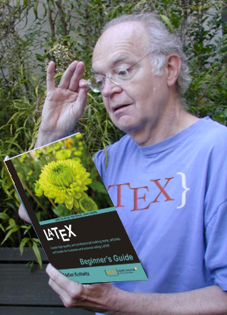
\includegraphics[width=0.3\textwidth]{input/images/donald.png}                   
\caption{Donald Knuth, Inventor Of \TeX{} 
typesetting system}
\hspace{-1.5em}
\end{figure}

Within the typesetting system, its name is styled as \LaTeX. The term 
\LaTeX{} refers only to the language in which documents are written, 
not to the editor used to write those documents. In order to create a 
document in \LaTeX, a .tex file must be created using some form of text 
editor. While most text editors can be used to create a \LaTeX{} document, 
a number of editors have been created specifically for working with \LaTeX.

\LaTeX{} is most widely used by mathematicians, scientists, 
engineers, philosophers, linguists, economists and other scholars in 
academia. As a primary or intermediate format, e.g., translating DocBook 
and other XML-based formats to PDF, \LaTeX{} is used because of the 
high quality of typesetting achievable by \TeX. The typesetting system 
offers programmable desktop publishing features and extensive facilities 
for automating most aspects of typesetting and desktop publishing, 
including numbering and cross-referencing, tables and figures, 
page layout and bibliographies.

\LaTeX{} is intended to provide a high-level language that
accesses the power of \TeX. \LaTeX{} essentially comprises a
collection of \TeX{} macros and a program to process \LaTeX documents. 
Because the \TeX{} formatting commands are very low-level, it is usually 
much simpler for end-users to use \LaTeX{}.


\subsection{Typesetting}
In preparing a \LaTeX{} document, the author 
specifies the logical structure using familiar concepts such as 
chapter, section, table, figure, etc., and lets the \LaTeX{} system 
worry about the presentation of these structures. It therefore 
encourages the separation of layout from content while still allowing 
manual typesetting adjustments where needed. 

\begin{verbatim}
\documentclass[12pt]{article}
\usepackage{amsmath}
\title{\LaTeX}
\date{}
\begin{document}
  \maketitle 
  \LaTeX{} is a document preparation system 
  for the \TeX{} typesetting program.
\end{document}
\end{verbatim}

\begin{figure}[!ht]
\centering
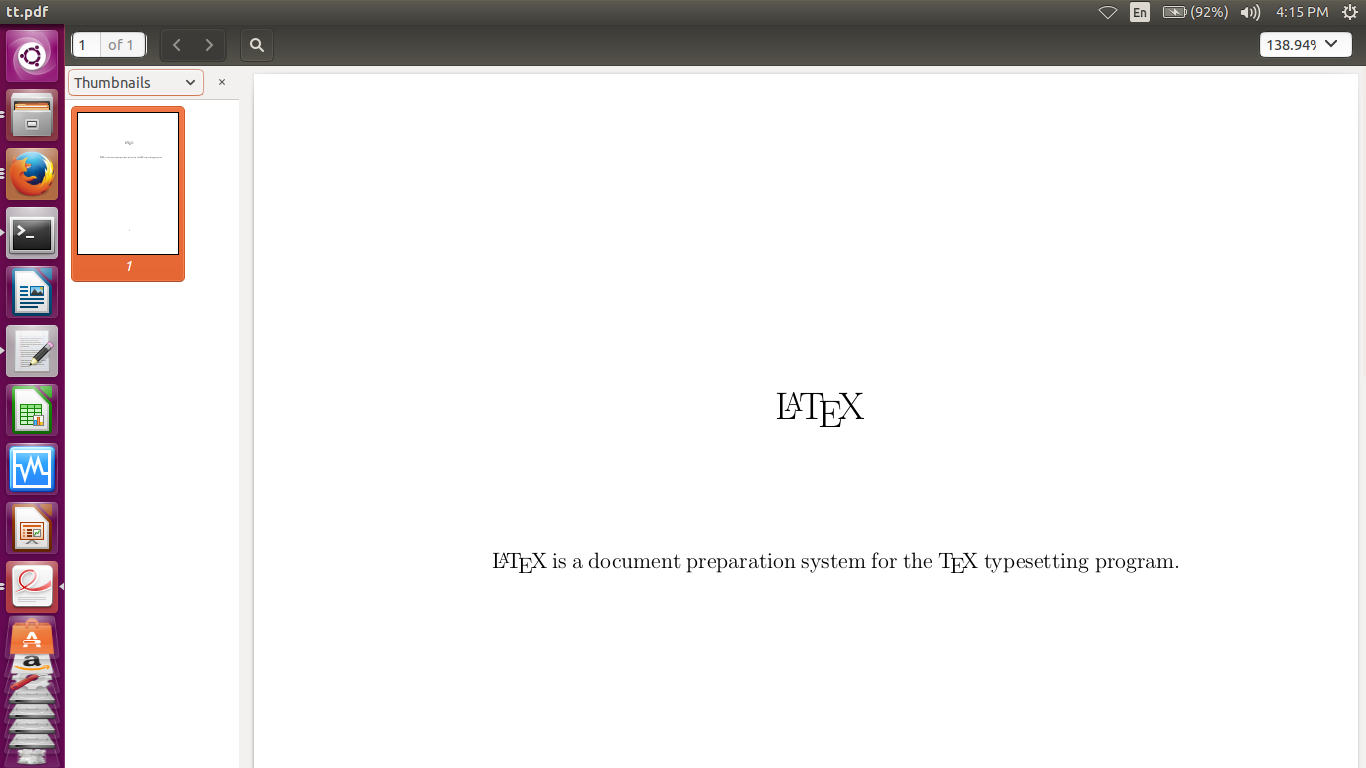
\includegraphics[width=0.5\textwidth]{input/images/la.png}
\caption{Output of the avove program}
\hspace{-1.5em}
\end{figure}

%\chapter{Requirements and Analysis}
%\input{input/req-n-ana.tex}
%Github\\
%IRC\\
%\LaTeX\\
%Lua\\

%

\section{Ubuntu: An open source OS}
\begin{figure}[!ht]
\centering

\includegraphics[width=0.3\textwidth]{input/images/ubu.png}
\caption{Ubuntu}
\hspace{-1.5em}
\end{figure}

During my training, I also got familiar with a great and open source Operating System, Ubuntu. Firstly, it was quite difficult for a regular MS Windows user to port to Ubuntu. I did all of my project work using this vast operating system. 
Ubuntu is a Debian-based Linux operating system, with Unity as its default desktop environment. It is based on free software and named after the Southern African philosophy of ubuntu (literally, "human-ness"), which often is translated as "humanity towards others" or "the belief in a universal bond of sharing that connects all humanity".\\

Ubuntu's goal is to be secure "out-of-the box". By default user's programs run with low privileges and cannot corrupt the operating system or other user's files. For increased security, the sudo tool is used to assign temporary privileges for performing administrative tasks, which allows the root account to remain locked and helps prevent inexperienced users from inadvertently making catastrophic system changes or opening security holes.\\




\begin{figure}[h!]
\centering 
\includegraphics[scale=1]{input/images/doxygen.jpeg}
\caption{Doxygen}
\end{figure}
\noindent Doxygen is a documentation generator, a tool for writing software reference 
documentation. The documentation is written within code, and is thus 
relatively easy to keep up to date. Doxygen can cross reference 
documentation and code, so that the reader of a document can easily 
refer to the actual code.

Doxygen supports multiple programming languages, especially C++, C, 
C\#, Objective-C, Java, Python, IDL, VHDL, Fortran and PHP.[2] Doxygen
 is free software, released under the terms of the GNU General Public 
License.\\

\section{Introduction To Doxygen}
\begin{itemize}
\item Requires very little overhead from the writer of the documentation. 
Plain text will do, Markdown is support, and for more fancy or structured 
output HTML tags and/or some of doxygen's special commands can be used.
\item Cross platform: Works on Windows and many Unix flavors (including 
Linux and Mac OS X).
\item Comes with a GUI frontend (Doxywizard) to ease editing the options 
and run doxygen. The GUI is available on Windows, Linux, and Mac OS X.
\item Automatically generates class and collaboration diagrams in HTML 
(as clickable image maps) and $\mbox{\LaTeX}$ (as Encapsulated PostScript 
images).
\item Allows grouping of entities in modules and creating a hierarchy 
of modules.
\item Doxygen can generate a layout which you can use and edit to change 
the layout of each page.
\item Can cope with large projects easily.
\end{itemize}
\subsection{Installation of Doxygen}
Doxygen can be installed using following commands:\\

\hspace{4pt} \$ git clone https://github.com/doxygen/doxygen.git

\hspace{4pt} \$ cd doxygen

\hspace{4pt} \$ ./configure

\hspace{4pt} \$ make

Documentation of this project.

\begin{figure}[h!]
	\centering 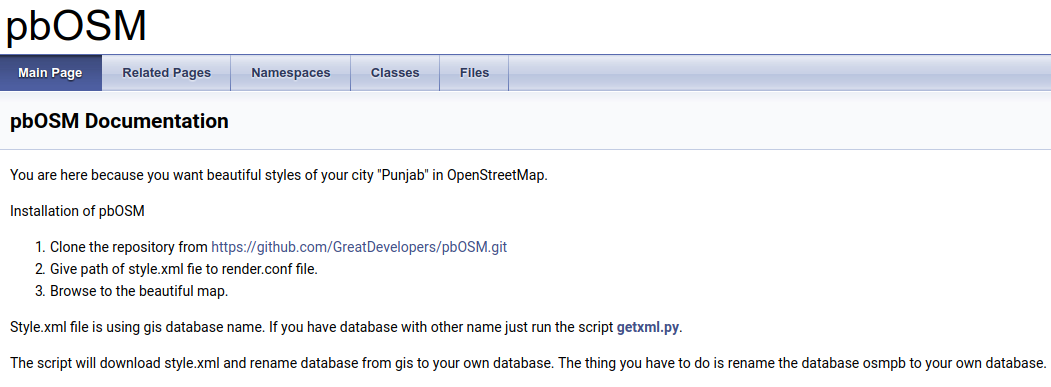
\includegraphics[scale=.4]{input/images/osm_doxygen.png}
	\caption{Main Page of pbOSM}
\end{figure}

\begin{figure}[h!]
	\centering 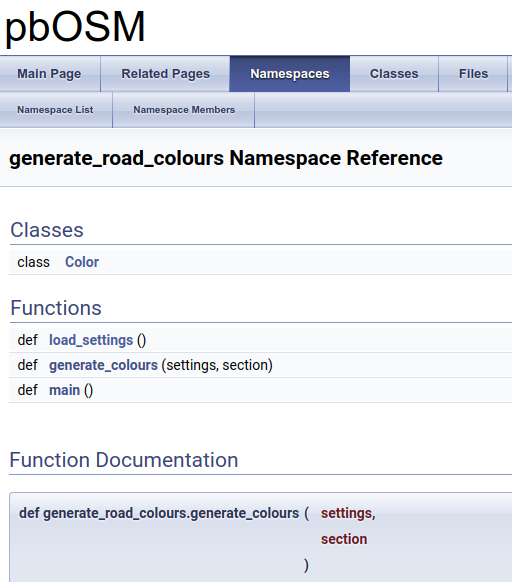
\includegraphics[scale=.6]{input/images/osm_doxygen1.png}
	\caption{Namespace documentation of pbOSM}
\end{figure}




\section{Introduction to \LaTeX}

\LaTeX, I had never heard about this term before doing this project,
but when I came to know about it's features, found it excellent. 
\LaTeX{ is a document markup language and document preparation system for the \TeX{} 
typesetting program. Within the typesetting system, its name is styled 
as \LaTeX.

\begin{figure}[!ht]
\centering
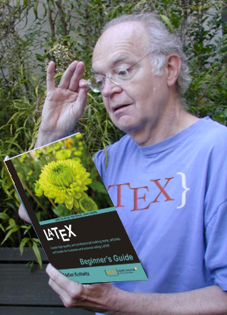
\includegraphics[width=0.3\textwidth]{input/images/donald.png}                   
\caption{Donald Knuth, Inventor Of \TeX{} 
typesetting system}
\hspace{-1.5em}
\end{figure}

Within the typesetting system, its name is styled as \LaTeX. The term 
\LaTeX{} refers only to the language in which documents are written, 
not to the editor used to write those documents. In order to create a 
document in \LaTeX, a .tex file must be created using some form of text 
editor. While most text editors can be used to create a \LaTeX{} document, 
a number of editors have been created specifically for working with \LaTeX.

\LaTeX{} is most widely used by mathematicians, scientists, 
engineers, philosophers, linguists, economists and other scholars in 
academia. As a primary or intermediate format, e.g., translating DocBook 
and other XML-based formats to PDF, \LaTeX{} is used because of the 
high quality of typesetting achievable by \TeX. The typesetting system 
offers programmable desktop publishing features and extensive facilities 
for automating most aspects of typesetting and desktop publishing, 
including numbering and cross-referencing, tables and figures, 
page layout and bibliographies.

\LaTeX{} is intended to provide a high-level language that
accesses the power of \TeX. \LaTeX{} essentially comprises a
collection of \TeX{} macros and a program to process \LaTeX documents. 
Because the \TeX{} formatting commands are very low-level, it is usually 
much simpler for end-users to use \LaTeX{}.


\subsection{Typesetting}
In preparing a \LaTeX{} document, the author 
specifies the logical structure using familiar concepts such as 
chapter, section, table, figure, etc., and lets the \LaTeX{} system 
worry about the presentation of these structures. It therefore 
encourages the separation of layout from content while still allowing 
manual typesetting adjustments where needed. 

\begin{verbatim}
\documentclass[12pt]{article}
\usepackage{amsmath}
\title{\LaTeX}
\date{}
\begin{document}
  \maketitle 
  \LaTeX{} is a document preparation system 
  for the \TeX{} typesetting program.
\end{document}
\end{verbatim}

\begin{figure}[!ht]
\centering
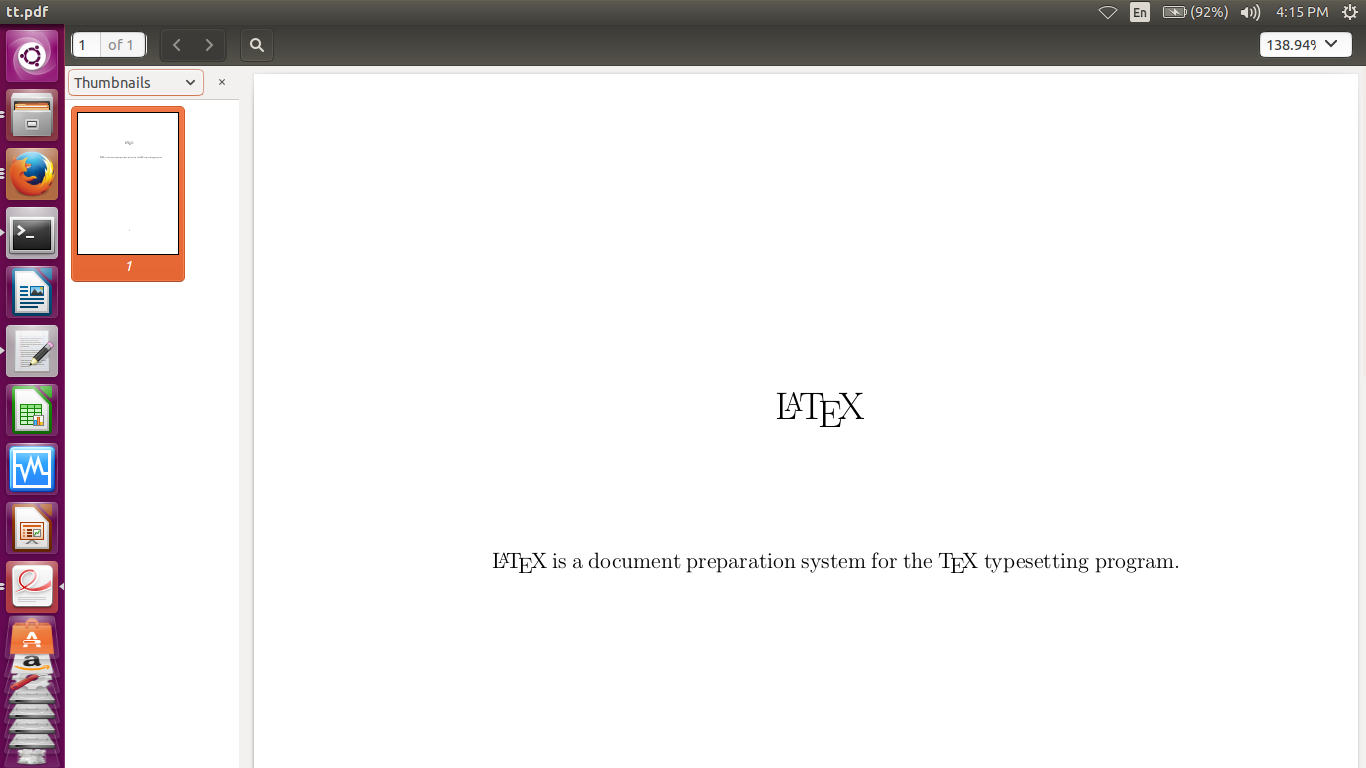
\includegraphics[width=0.5\textwidth]{input/images/la.png}
\caption{Output of the avove program}
\hspace{-1.5em}
\end{figure}


\section{Introduction to Github}
\begin{figure}[!ht]
\centering

\includegraphics[width=0.3\textwidth]{/home/amisha/gitt/6-weeks-report/input/images/github.jpg}                   
\caption{Github Logo}
\hspace{-1.5em}
\end{figure}
\leavevmode\\
GitHub is a Git repository web-based hosting service which offers all of the functionality of Git as well as adding many of its own features. Unlike Git which is strictly a command-line tool, Github provides a web-based graphical interface and desktop as well as mobile integration. It also provides access control and several collaboration features such as wikis, task management, and bug tracking and feature requests for every project.\\

GitHub offers both paid plans for private repo handle everything from small to very large projects with speed and efficiency. ositories, and free accounts, which are usually used to host open source software projects. As of 2014, Github reports having over 3.4 million users, making it the largest code host in the world.\\

GitHub has become such a staple amongst the open-source development community that many developers have begun considering it a replacement for a conventional resume and some employers require applications to provide a link to and have an active contributing GitHub account in order to qualify for a job.\\

The Git feature that really makes it stand apart from nearly every
other Source Code Management (SCM) out there is its branching model.\\
\\
Git allows and encourages you to have multiple local branches that can
be entirely independent of each other. The creation, merging, and
deletion of those lines of development takes seconds.\\ \\
This means that you can do things like:
\begin{itemize}
\item Frictionless Context Switching.\\ Create a branch to try out an
idea, commit a few times, switch back to where you branched from,
apply a patch, switch back to where you are experimenting, and merge
it in.
\item Role-Based Code lines. \\ Have a branch that always contains only
what goes to production, another that you merge work into for testing,
and several smaller ones for day to day work.
\item Feature Based Work flow. \\ Create new branches for each new
feature you're working on so you can seamlessly switch back and forth
between them, then delete each branch when that feature gets merged
into your main line.
\item Disposable Experimentation.\\  Create a branch to experiment in,
realize it's not going to work, and just delete it - abandoning the
work—with nobody else ever seeing it (even if you've pushed other
branches in the meantime).
\end{itemize}
Notably, when you push to a remote repository, you do not have to push
all of your branches. You can choose to share just one of your
branches, a few of them, or all of them. This tends to free people to
try new ideas without worrying about having to plan how and when they
are going to merge it in or share it with others.\\ \\
There are ways to accomplish some of this with other systems, but the
work involved is much more difficult and error-prone. Git makes this
process incredibly easy and it changes the way most developers work
when they learn it.

\subsection{What is Git?}
\begin{figure}[!ht]
\centering

\includegraphics[width=0.3\textwidth]{/home/amisha/gitt/6-weeks-report/input/images/git.jpg}                   
\caption{Git Logo}
\hspace{-1.5em}
\end{figure}
Git is a distributed revision control and source code management (SCM) system with an emphasis on speed, data integrity, and support for distributed, non-linear workflows. Git was initially designed and developed by Linus Torvalds for Linux kernel development in 2005, and has since become the most widely adopted version control system for software development.\\

As with most other distributed revision control systems, and unlike most client–server systems, every Git working directory is a full-fledged repository with complete history and full version-tracking capabilities, independent of network access or a central server. Like the Linux kernel, Git is free and open source software distributed under the terms of the GNU General Public License version 2 to handle everything from small to very large projects with speed and efficiency.\\

Git is easy to learn and has a tiny footprint with lightning fast performance. It outclasses SCM tools like Subversion, CVS, Perforce, and ClearCase with features like cheap local branching, convenient staging areas, and multiple workflows.\\

\subsection{Installation of Git}

Installation of git is a very easy process.
The current git version is: 2.0.4.
Type the commands in the terminal:\\\\
\emph{
\$ sudo apt-get update\\\\
\$ sudo apt-get install git\\\\}
This will install the git on your pc or laptop.

\subsection{Various Git Commands}

Git is the open source distributed version control system that facilitates GitHub activities on your laptop or desktop. The commonly used Git command line instructions are:-\\

\subsubsection{Create Repositories}
Start a new repository or obtain from an exiting URL

\begin{description}

\item [\$ git init [ project-name]]\\
Creates a new local repository with the specified name
\item [\$ git clone [url]]\\
Downloads a project and its entire version history\\

\end{description}


\subsubsection{Make Changes}
Review edits and craft a commit transaction

\begin{description}

\item [\$ git status] \leavevmode \\
Lists all new or modified files to be committed

\item [\$ git diff] \leavevmode \\
Shows file differences not yet staged

\item [\$ git add [file]]\\
Snapshots the file in preparation for versioning

\item [\$ git commit -m "[descriptive message]"]\\
Records file snapshots permanently in version history\\

\end{description}


\subsubsection{Group Changes}
Name a series of commits and combine completed efforts

\begin{description}

\item [\$ git branch] \leavevmode \\
Lists all local branches in the current repository

\item [\$ git branch [branch-name]]\\
Creates a new branch

\item [\$ git checkout [branch-name]]\\
Switches to the specified branch and updates the working directory

\item [\$ git branch -d [branch-name]]\\
Deletes the specified branch\\

\end{description}


\subsubsection{Synchronize Changes}
Register a repository bookmark and exchange version history

\begin{description}

\item [\$ git fetch [bookmark]]\\
Downloads all history from the repository bookmark

\item [\$ git merge [bookmark]/[branch]]\\
Combines bookmark’s branch into current local branch

\item [\$ git push [alias][branch]]\\
Uploads all local branch commits to GitHub

\item [\$ git pull] \leavevmode \\
Downloads bookmark history and incorporates changes

\end{description}



\section{Introduction to Reveal-js \& Reveal-md}
\begin{figure}[!ht]
\centering

\includegraphics[width=0.3\textwidth]{input/images/reveal.png}                   
\caption{MD \& JS}
\hspace{-1.5em}
\end{figure}
Reveal-js is one of the framework of Javascript. This can be used for presentations purpose.\\
Now before going to reveal-md lets talk about some fundamental things.\\
What is a Markup language?\\
Markup languages are designed for the processing, definition and presentation of text. The language specifies code for formatting, both the layout and style, within a text file. HTML and Markdown  is an example of a widely known and used markup language.\\
Markdown is a lightweight Markup Language with simple plain text formatting syntax designed so that it can be converted to HTML and many other formats. It is created by  John Gruber. It had '.md' or '.markdown' extention.\\
"Markdown is a text-to-HTML conversion software tool written in Perl for web writers."\\
Moreover, to enable markdown feature of reveal.js, we need reveal-md. The Markdown feature of reveal.js is awesome, and has an easy (and configurable) syntax to separate slides. Use three dashes surrounded by two blank lines.\\
\subsection{Installation of reveal-md}
Installation of reveal-md is a very easy process.
Type the commands in the terminal:\\\\
\emph{
\$ sudo apt-get install npm\\\\
\$ sudo apt-get install nodejs-legacy\\\\
\$ sudo npm install -g reveal-md\\\\}
This will install reveal-md on your pc or laptop.



\section{Working with Experimental Server}
\begin{figure}[!ht]
\centering

\includegraphics[width=0.3\textwidth]{input/images/ser.png}                   
\caption{Server Communication}
\hspace{-1.5em}
\end{figure}
I had also done the whole project on ubuntu experimental server and had also learnt about making your system a server.\\
What is a Remote Server?\\
In simple words its nothing much but a Computer that is not attached to a user’s keyboard but over which he or she has some degree of control (like can see data of that computer, can retrieve or send data etc.)\\
For going deep you need to know about ssh (Secure Shell). I had  written about it in my old blogs. You can Google it too.\\
I had done it using SSH. There are few terms related to this :\\
\begin{itemize}
\item SSH: It is a Secure Socket Shell, is a network protocol that provides administrators with a secure way to access a remote computer.
\item MOSH: It is a software tool used to connect from a client computer to a server over the Internet, to run a remote terminal. 
\item Tmux: tmux is basically a terminal multiplexer. It is used so that within
one terminal window we can open multiple windows and split-views.
\item OpenSSH: It is a freely available version of the Secure Shell (SSH) protocol family of tools for remotely controlling or transferring files between computers. Traditional tools used to accomplish this is telnet which is not much secure.
\end{itemize}

In Unix, you can use SCP (the scp command) to securely copy files and directories between remote hosts without starting an FTP session or logging into the remote systems explicitly. \\
The scp command uses SSH to transfer data, so it requires a password.\\\\
Some of the useful commands in this for checking errors or for other purposes are: \\
\begin{itemize}
\item ll: This command is used to list the detail information of files and folder of a current directory. 
\item tail -f error.log: This is used for checking errors.
\item sudo apt-get install openssh-server
\item sudo vim /etc/ssh/sshdconfig \\
(To edit this as per your preferences. But first take a backup of this file for later default configurations if needed.)
\item sudo restart ssh \\
(To check your ssh daemon is running or not.)

\item ssh user@hostip \\
(To enter into a remote server from some other system. )
\end{itemize}

 

%\section{Certificate Genertion System}

Apart from the major project i.e OSM I have done another project "Certificate Generation System".

Certificate Generation System is a portable application used to Generate Certificate for single candidate providing his/her details along with image,
As well as for Batch/Number of candidates by simply providing the CSV format file (containing details of every candidate) along with candidate images.

CSV(Character Separated File) is a simple file format used to store tabular data, such as a spreadsheet or database. Files in the CSV format can be imported to and exported from programs that store data in tables, such as Microsoft Excel or OpenOffice Calc.

INSTALLATION/SETUP

This application is a portable application used to Generate Certificate for single candidate providing his/her details along with image,
As well as for Batch/Number of candidates by simply providing the CSV format file (containing details of every candidate) along with candidate images in a compressed (tar.gz or zip) folder.
Requirements(automatically installed during setup)

    Apache web server
    php interpreter
    unoconv
    python3-uno

USER MANUAL

As the Name "Certificate Generation System" Implies this application is used to generate certificate in an automated manner in few steps:

    Select Design from the images shown on the first page. ( Put mouse pointer over the image to see larger view. )

\begin{figure}[!ht]
\centering
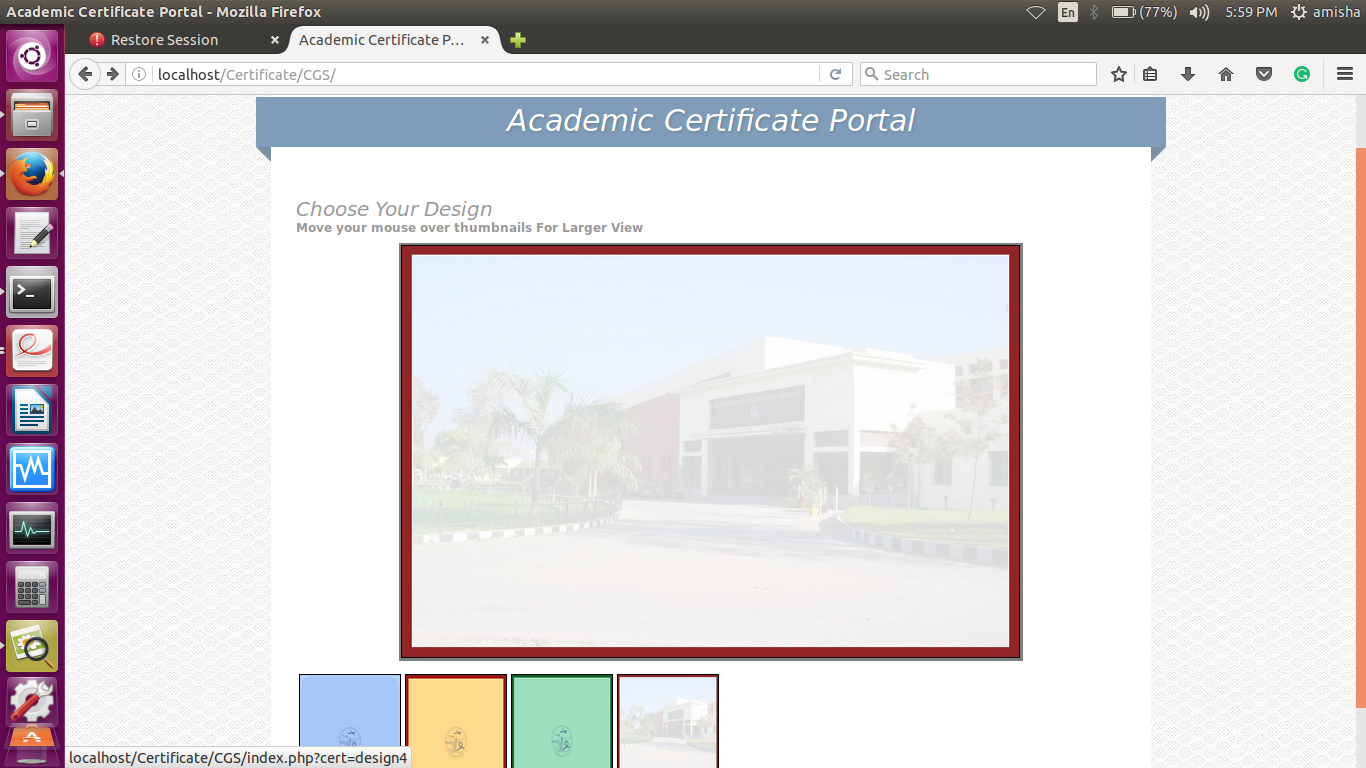
\includegraphics[width=0.7\textwidth]{input/images/cgs/cgs1.png}
\caption{Academic Portal}
\hspace{-1.5em}
\end{figure}


    Next Page will be page for entering Institute Details.


    Fill in the details of institution for which the certificate(s) is to be made.

    Place mouse pointer over Input box te see an example for that input.
\begin{figure}[!ht]
\centering
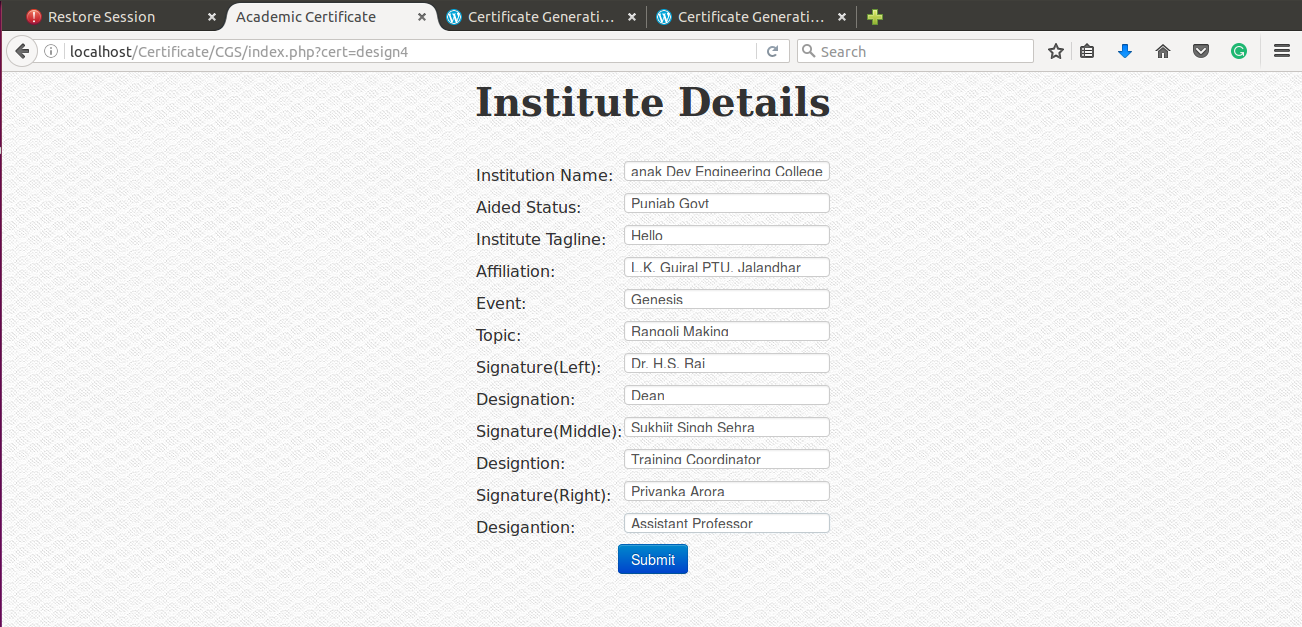
\includegraphics[width=0.7\textwidth]{input/images/cgs/cgs2.png}                  
\caption{Institute Details}
\hspace{-1.5em}
\end{figure}


    Next page will show two options

    Manual Entry -> Select it for Generating Certificate for Single candidate.

    Upload Csv File -> Select it for Generating certificate for more than 1 candidate by providing their details in Csv file.
    Manual Entry
\begin{figure}[!ht]
\centering
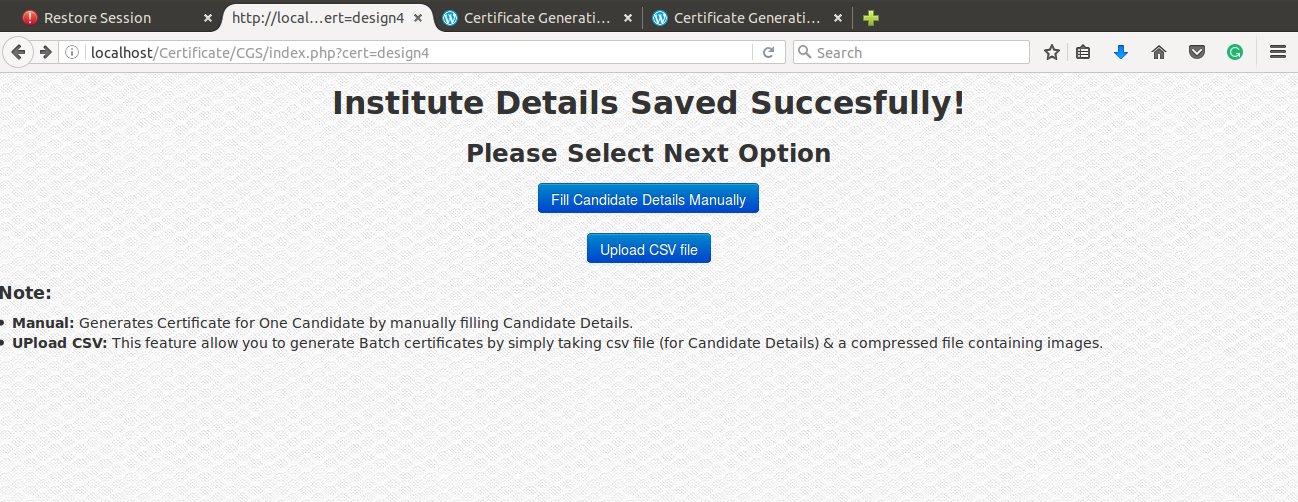
\includegraphics[width=0.7\textwidth]{input/images/cgs/cgs3.png}                  
\caption{Select Manual Option}
\hspace{-1.5em}
\end{figure}

    On Selecting Manual Entry Next page will open containing input boxes for candidate Details.

    Enter the details and select the image also.

    Live Image Selector

    Next you will be displayed your selected image and a selection box.

\begin{figure}[!ht]
\centering
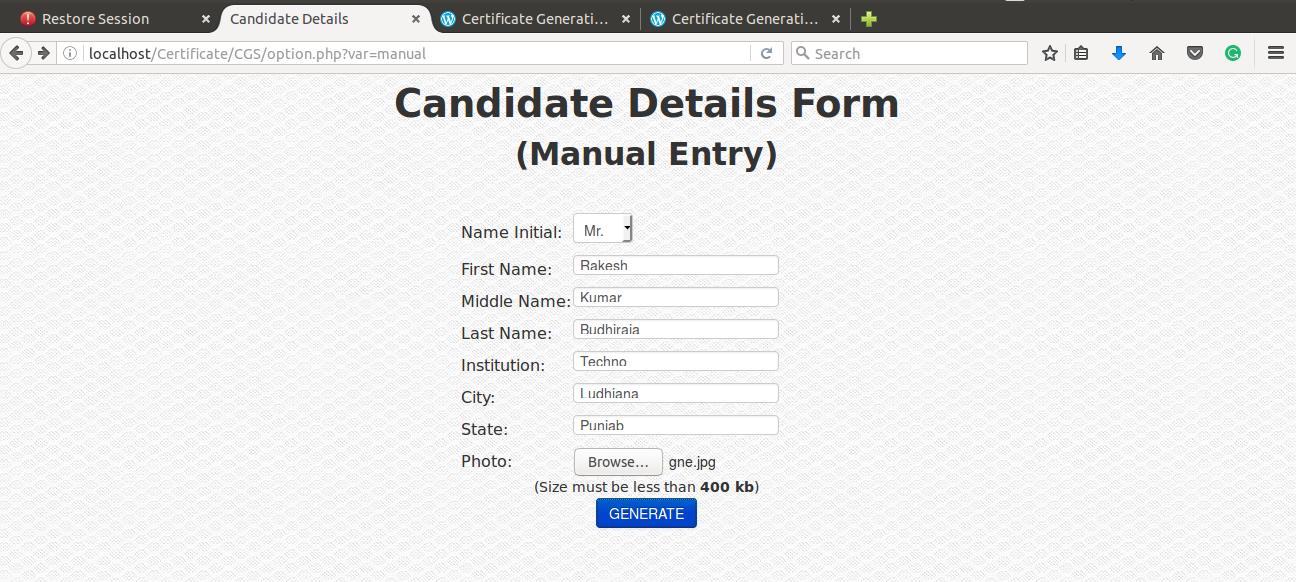
\includegraphics[width=0.7\textwidth]{input/images/cgs/cgs4.png}                  
\caption{Candidate Details Form}
\hspace{-1.5em}
\end{figure}

    Resize and move the selection box to desired position and size.

\begin{figure}[!ht]
\centering
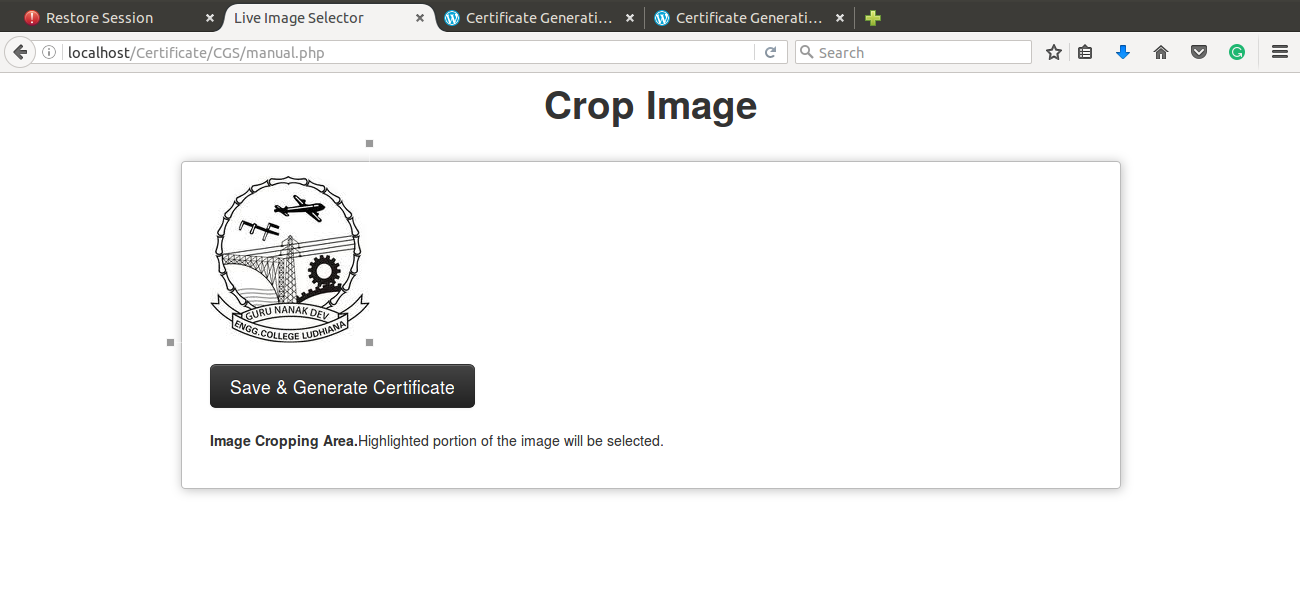
\includegraphics[width=0.7\textwidth]{input/images/cgs/cgs5.png}                  
\caption{Crop Image}
\hspace{-1.5em}
\end{figure}

    Download

    Thats it your certificate is generated and can be downloaded in two formats

    -> odt ('O'penOffice 'D'ocument 'T'ext)

    -> pdf ('P'ortable 'D'ocument 'F'ormat)

\begin{figure}[!ht]
\centering
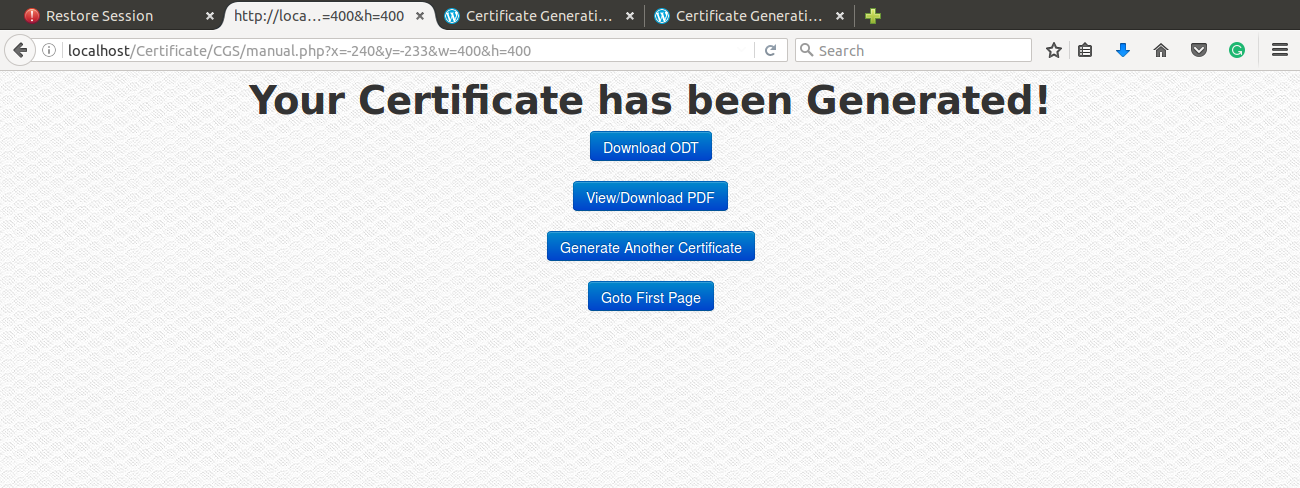
\includegraphics[width=0.7\textwidth]{input/images/cgs/cgs6.png}                  
\caption{Download Certificate}
\hspace{-1.5em}
\end{figure}

\begin{figure}[!ht]
\centering
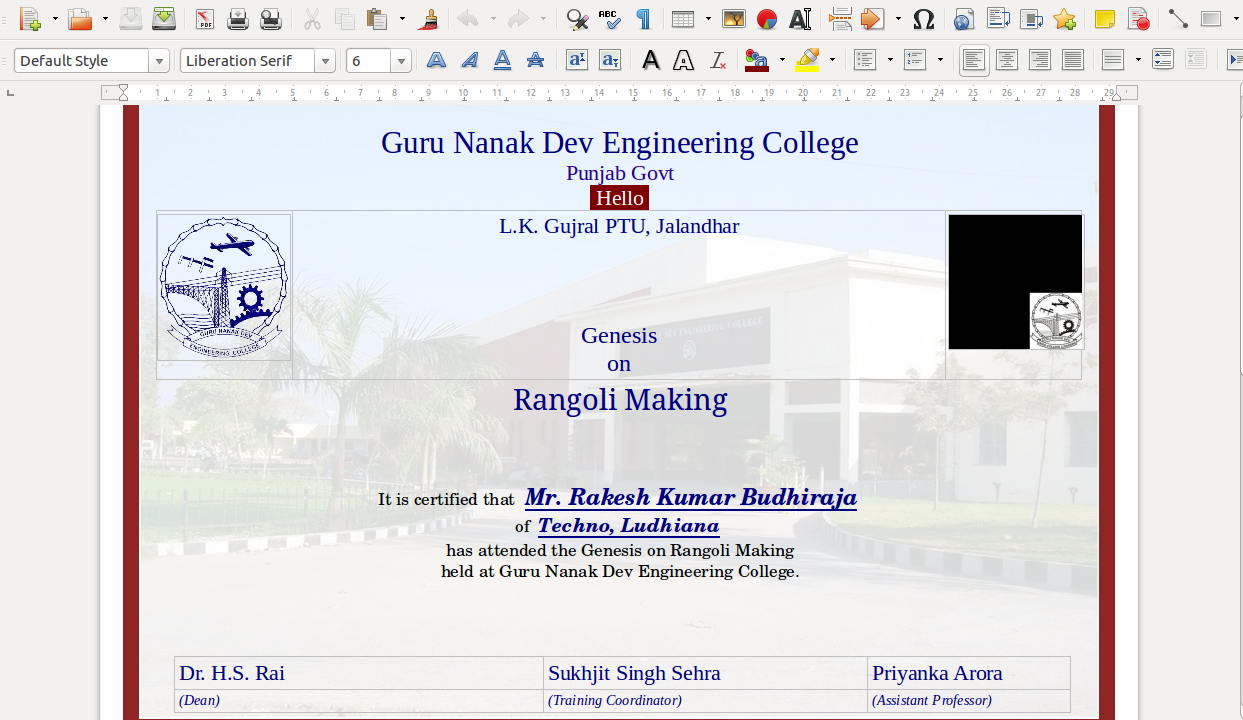
\includegraphics[width=0.7\textwidth]{input/images/cgs/cgs8.png}                 
\caption{Certificate odt file}
\hspace{-1.5em}
\end{figure}


    Also by clicking on "Generate Another Ceritificate" you can generate another certificate

    with same design & institute details and different Candidate Details.

    And by clicking on "Goto First Page" you can again start from Design Selection Page.
    Upload csv file

    On selecting 'Upload csv File' Next page will open containing the conditions for the files

    to be uploaded for certificate generation.
\begin{figure}[!ht]
\centering
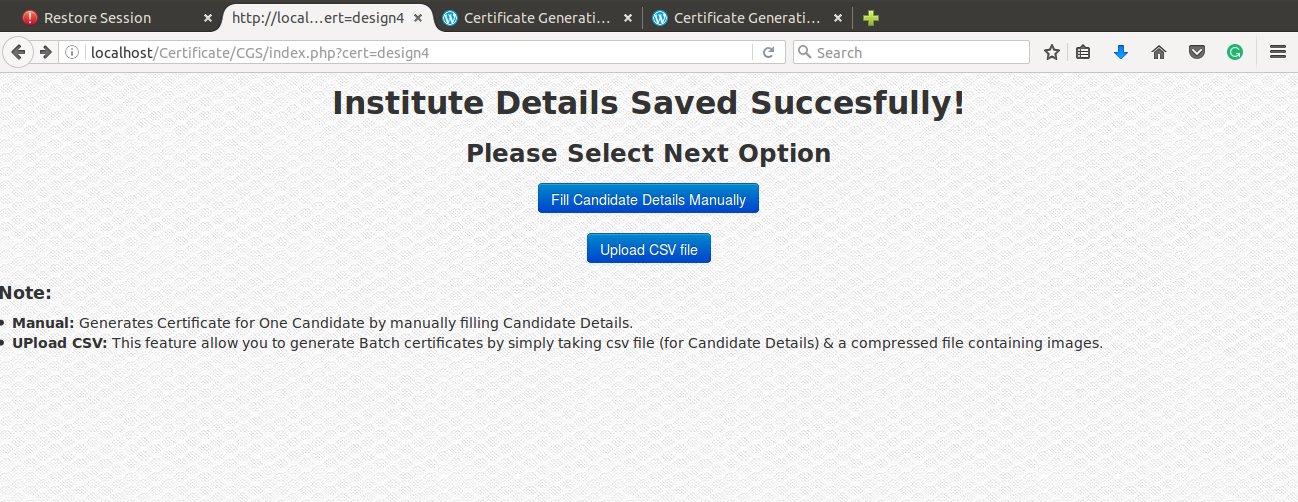
\includegraphics[width=0.7\textwidth]{input/images/cgs/cgs3.png}                  
\caption{Choose csv Option}
\hspace{-1.5em}
\end{figure}
    A sample file can be downloaded from the link provided in the 'Note' in the instructions on page.

    Sample file is a zip file named sample.zip containing the csv file and tar.gz file for images.

    Extract it and then sample certificates can be produced using 'sample.csv' and 'images.tar.gz' files.

\begin{figure}[!ht]
\centering
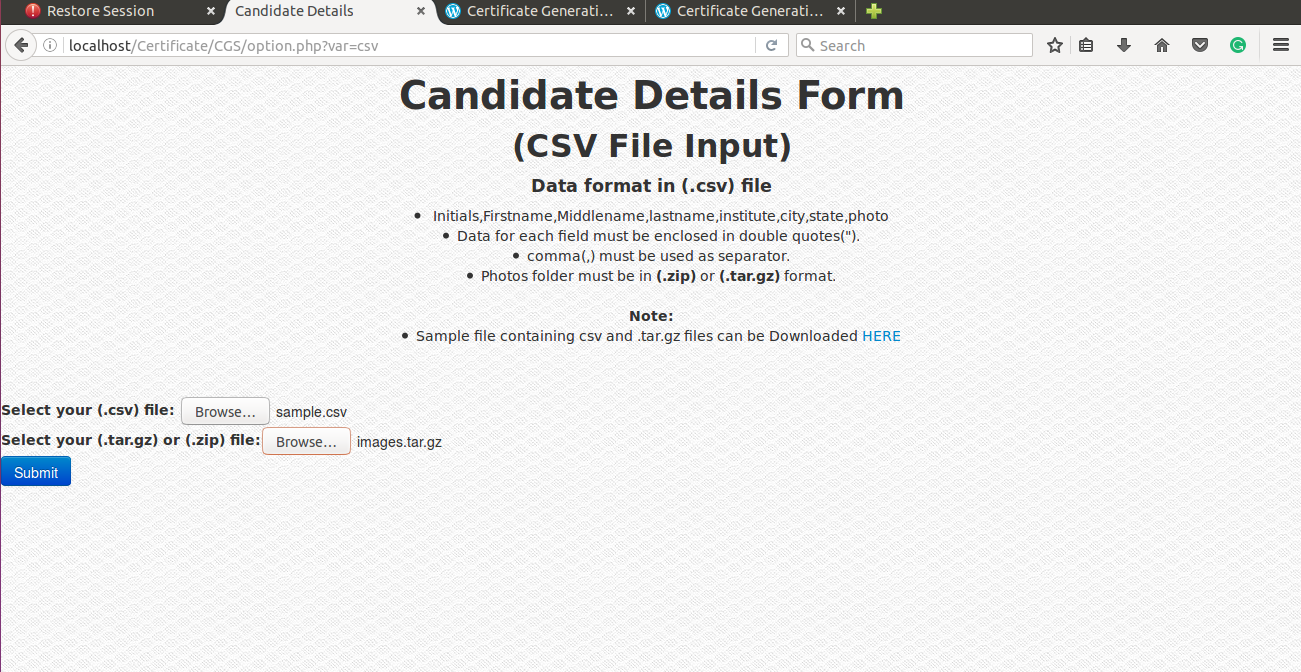
\includegraphics[width=0.7\textwidth]{input/images/cgs/cgs9.png}                 
\caption{Candidate Details Form}
\hspace{-1.5em}
\end{figure}


    That's it your certificate file is produced for all the candidates provided in the csv data file.

Produced Certificate file can be downloaded in two formats again.

-> odt ('O'penOffice 'D'ocument 'T'ext)

-> pdf ('P'ortable 'D'ocument 'F'ormat)
\begin{figure}[!ht]
\centering
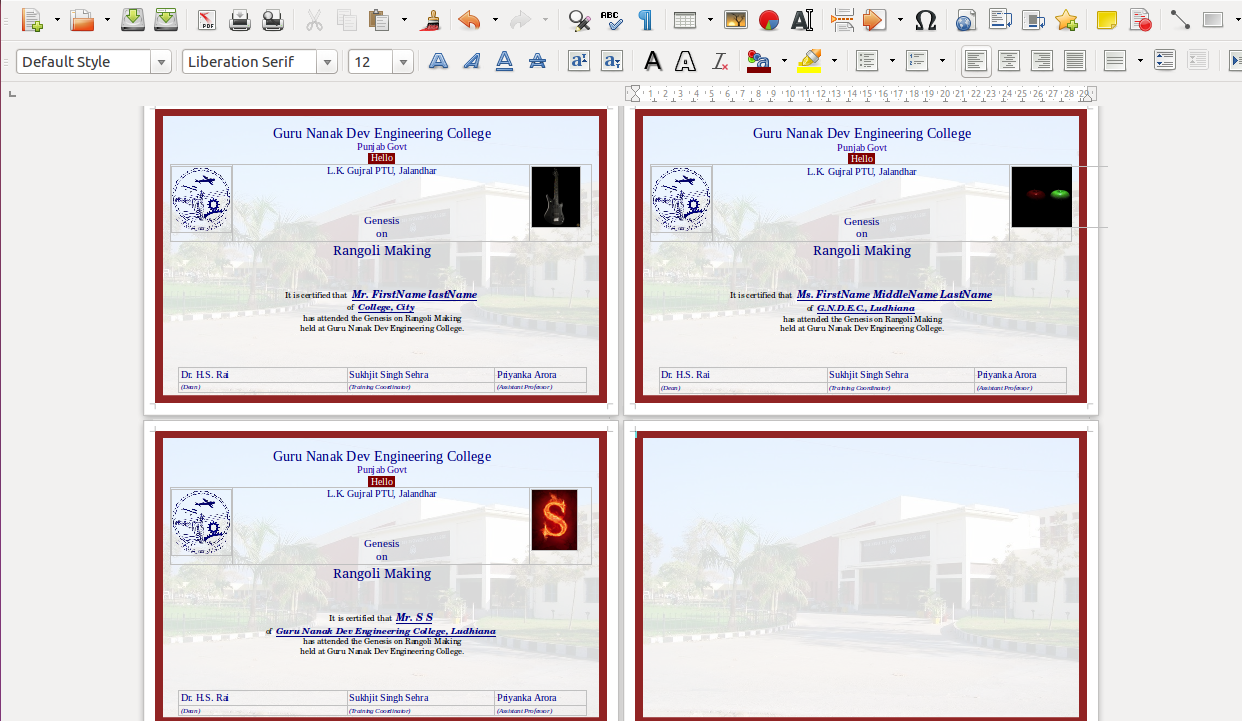
\includegraphics[width=0.7\textwidth]{input/images/cgs/cgs14.png}                  
\caption{Odt file through csv}
\hspace{-1.5em}
\end{figure}

\section{OSM and its Components }
It is a collaborative project to create a free editable map of the world.
Now ,before beginning to make your own tile server, review some termonologies.
\begin{figure}[ht]
\centering 
\includegraphics[scale=0.6]{input/images/index.jpeg}
\caption{OpenStreetMap logo}
\end{figure}

\subsection{Benifits Of Own Tile Server}
 OSM map is accessible even when internet provider is down or when the power is off or both. It won't take much for to see the benefit of having your own piece of OpenStreetMap infrastructure.\\
Now it's turn to install, setup and configure all the necessary software to operate own tile server. All the instructions are illustrated in blog "https://amisha2016.wordpress.com"\\
These instructions build what OpenStreetMap calls a "tile server". That is, a computer that uses the OSM data set to create map images that are suitable for a website. Not every OpenStreetMap function is supported, but you will be able to create a local map, keep it up to date and customize it for your own purposes.
\begin{figure}[!ht]
\centering

\includegraphics[width=0.4\textwidth]{input/images/index.png}                   
\caption{Postgresql}
\hspace{-1.5em}
\end{figure}


\subsection{Postgresql / postgis}
PostGIS is a spatial database extender for PostgreSQL object-relational database. It adds support for geographic objects allowing location queries to be run in SQL.\\
Most spatial databases allow representing simple geometric objects such as points, lines and polygons. Some spatial databases handle more complex structures such as 3D objects, topological coverages, linear networks, and TINs.\\
On Ubuntu there are pre-packaged versions of both postgis and postgresql, so these can simply be installed via the Ubuntu package manager.\\
\subsection{Osm2pgsql}
 osm2pgsql is under active development and is best compiled from source.\\
osm2pgsql is a command-line based program that converts OpenStreetMap data to postGIS-enabled PostgreSQL databases.\\
Mapnik is an open source mapping toolkit for desktop- and server-based map rendering, written in C++.\\
One of its many users is the OpenStreetMap project (OSM), which uses it in combination with an Apache Web Server module (mod\_tile) to render tiles that make up the OSM ‘Slippy Map’ Layer.\\
\begin{figure}[!ht]
\centering
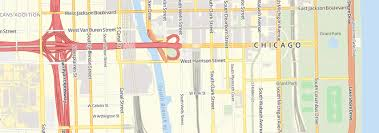
\includegraphics[width=0.7\textwidth]{input/images/bright.jpeg}                   
\caption{Openstreetmap-carto Style}
\hspace{-1.5em}
\end{figure}



\subsection{Openstreetmap-carto}
Openstreetmap-carto is a sensible starting point for quickly making beautiful maps based on an OpenStreetMap database. It is written in the Carto styling language and can be opened as a project in TileMill.\\
The style is still a work in progress and you are encouraged to use the issue tracker to note missing features or problems with the current implementation.\\
\subsection{OpenLayer.js}
OpenLayers makes it easy to put a dynamic map in any web page. It can display map tiles, vector data and markers loaded from any source. OpenLayers has been developed to further the use of geographic information of all kinds. It is completely free.\\
\subsection{Geographic Information Systems (GIS)}
GIS is a computer system for capturing, storing, checking, and displaying data related to positions on Earth’s surface. GIS can show many different kinds of data on one map. This enables people to more easily see, analyze, and understand patterns and relationships\\
The Global Positioning System (GPS) is a space-based navigation system that provides location and time information in all weather conditions, anywhere on or near the Earth where there is an unobstructed line of sight to four or more GPS satellites.\\


%\chapter{Design}
%\section{DFDs}
A data flow diagram (DFD) is a graphical representation of the "flow" of data through an information system, modeling its process aspects. A DFD is often used as a preliminary step to create an overview of the system, which can later be elaborated. DFDs to serve a tile is as following-:
\begin{figure}[h!]
\centering
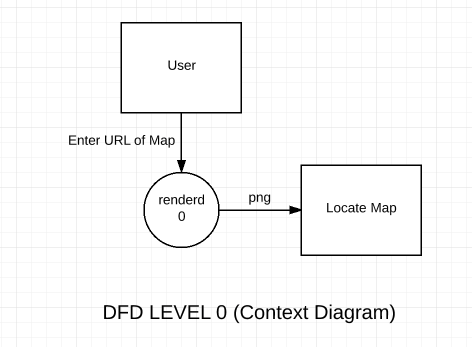
\includegraphics[scale=0.6]{input/images/DFD_0.png}
\caption{Data Flow Diagram Level 0}
\end{figure}
\begin{figure}[h!]
	\centering
	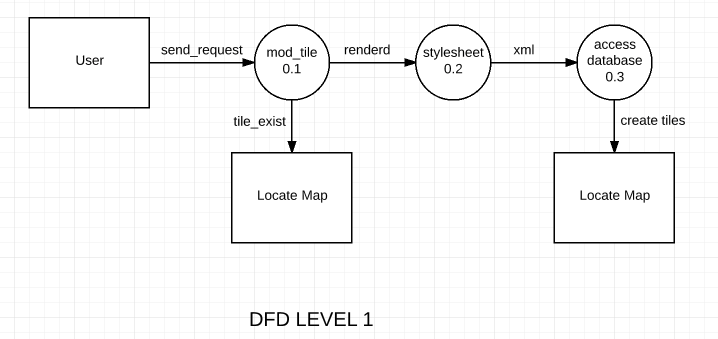
\includegraphics[scale=0.6]{input/images/DFD_1.png}
	\caption{Data Flow Diagram Level 1}
\end{figure}
\begin{figure}[h!]
	\centering
	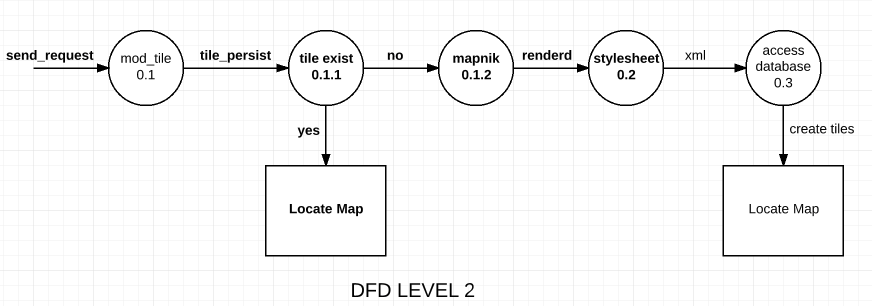
\includegraphics[scale=0.6]{input/images/DFD_2.png}
	\caption{Data Flow Diagram Level 2}
\end{figure}

\section{Flowchart}
A flowchart is a type of diagram that represents an algorithm, work flow or process, showing the steps as boxes of various kinds, and their order by connecting them with arrows
and following are flowchart of showing flow of control and Data in the software-:

\begin{figure}[h!]
	\centering
	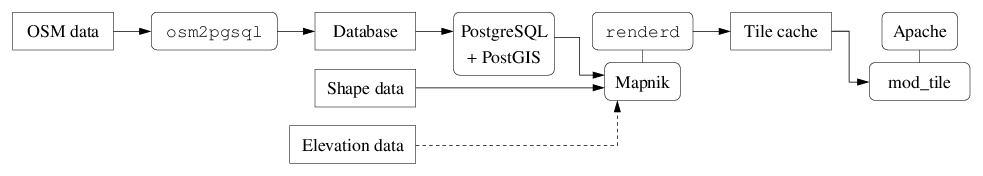
\includegraphics[scale=0.6]{input/images/osmserv.png}
	\caption{Data Flow Of Whole System}
\end{figure}



\begin{figure}[h!]
\centering
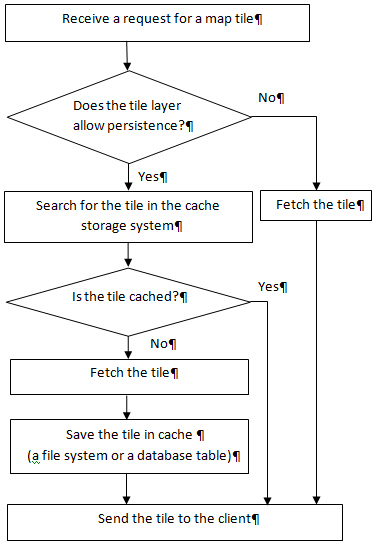
\includegraphics[scale=0.9]{input/images/fetch.jpg}
\caption{Flow Chart to Serve a Tile}
\end{figure}
\hspace{-1.7em}



\section{Problem Formulation}
Geographical data (geo data) is not free in many parts of the world.\\
Because that data is copyrighted and owned by multiple organisations like the Ordnance Survey. Google/whoever just licenses it. If we were to use it, we'd have to pay for it. \\
\noindent "OpenStreetMap is a free editable map of the whole world. It is made by people like you." Which means the database will always be subject to the whims, experimentation, and mistakes of the community. This is precisely OSM's strength since, among other things, it allows our data to quickly accommodate changes in the physical world.\\
\noindent By making your system an OSM tile server not only you can edit the map but can use it offline also. You can change the styling of the map like color of the roads fonts style and amny more as per your requirments. 


\section{Dependencies}
%\subsection{Hardware Requirements}
\begin{itemize}
\item Operating System: Linux/Windows
\item Processor Speed: 512KHz or more
\item RAM: Minimum 2GB
\item Library: Mapnik
\item Modules: Mod\_tile
\item Compiler: CartoCSS
\item Stylesheet: OSMBright
\item Programming Language: C++, Python
\end{itemize}
%\subsection{Software Requirements}
%\begin{itemize}
%\item Library: Mapnik
%\item Modules: Mod\_tile
%\item Compiler: CartoCSS
%\item Stylesheet: OSMBright 
%\item Programming Language: C++, Python 
%\end{itemize}

\section{Methodology}
\begin{itemize}
\item Studying various methods available to solve different problems of numerical analysis.
\item Deciding various input and output parameters of methods.
\item Making the approach modular 
\item Styling the map.
\item Generating documentation
\end{itemize}

\section{Project Work} 
\textbf{Studied Previous System:}\\
Before starting the project, \\\\
\textbf{Learn Linux:}\\
Before starting with project, we have to install various things to make our system an OSM server. So, for that you should know terminal commands because I gonna explain it for Ubuntu only. It is possible on other OS also but you have to work it own. I have provided some basic command also for Linux. \\\\
\textbf{Learn Postgresql:}\\
 We have to go through the basics of postgresql(database) also, such that there
should not be any problem proceeding with project.\\\\
\textbf{Make or Cmake}\\
The softwares like mapnik, mod\_tile, osm2pqsql, are compiled through the Cmake which is basically language. So, we should the basics of it.
\\\\
\textbf{Languages:}\\
We should the basics of the languages like C++, javascript, python etc for manuplating the stylying and rendering of the map.\\\\
\textbf{Input:}\\
Input values are taken from user or default values defined in the file are used.\\\\
\textbf{Output:}\\
According to input values we will get the particular location of the map.


%\chapter{Implementation}
%\input{input/implement.tex}
\newgeometry{textwidth=16cm,textheight=26cm,voffset=-2cm,bottom=0cm}
\newpage
\chapter*{Introduction To Organisation}
%\chapter{Introduction To Organisation}

\begin{figure}[ht]
\centering
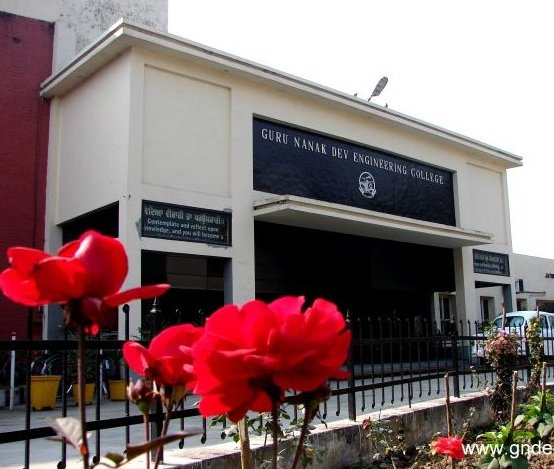
\includegraphics[scale=0.5]{/home/amisha/gitt/6-weeks-report/input/images/gndec.jpg}
\caption{Guru Nanak Dev Engineering College}
\end{figure}
\hspace{-1.7em}
 I had my Six Weeks Training at TCC-Testing And Consultancy Cell, GNDEC Ludhiana. Guru Nanak Dev Engineering College was established by the Nankana Sahib Education Trust Ludhiana. The Nankana Sahib Education Trust i.e NSET
was founded in memory of the most sacred temple of Sri Nankana Sahib, birth place
of Sri Guru Nanak Dev Ji. With the mission of Removal of Economic Backwardness
through Technology Shiromani Gurudwara Parbandhak Committee i.e SGPC started a
Poly technical was started in 1953 and Guru Nanak Dev Engineering College was established in 1956.\\
NSET resolved to uplift Rural areas by admitting 70\% 
of students from these rural
areas ever year. This commitment was made to nation on 8th April, 1956, the day
foundation stone of the college building was laid by Dr. Rajendra Prasad Ji, the First
President of India. The College is now ISO 9001:2000 certified.\\
Guru Nanak Dev Engineering College campus is spread over 88 acres of prime land
about 5 Kms from Bus Stand and 8 Kms from Ludhiana Railway Station on Ludhiana-Malerkotla Road. The college campus is well planned with beautifully laid out tree plantation, pathways, flowerbeds besides the well maintained sprawling lawns all around. It
has beautiful building for College,Hostels,Swimming Pool,Sports and Gymnasium Hall
Complex, Gurudwara Sahib, Bank, Dispensary, Post Office etc. There are two hostels
for boys and one for girls with total accommodation of about 550 students. The main
goal of this institute is:\\
\begin{itemize}
\item To build and promote teams of experts in the upcoming specialisations.
\item To promote quality research and undertake research projects keeping in view their relevance to needs and requirements of technology in local industry.
\item To achieve total financial independence.
\item To start online transfer of knowledge in appropriate technology by means of establishing multipurpose resource centres.
\end{itemize}
\section{Testing and Consutancy Cell}

My Six Weeks Institutional Training was done by me at TCC i.e Testing And
Consultancy Cell,
GNDEC Ludhiana under the guidance of Dr. H.S.Rai Dean Testing and Consultancy Cell.
Testing and Consultancy Cell was established in the year 1979 with a basic aim to produce
quality service for technical problems at reasonable and affordable rates as a service to society
in general and Engineering fraternity in particular.\\
\begin{figure}[ht]
\centering
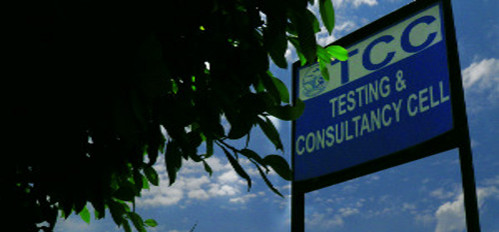
\includegraphics[scale=0.7]{/home/amisha/gitt/6-weeks-report/input/images/aw.jpg}
\caption{Testing and Consultancy Cell}
\end{figure}
\hspace{-1.7em} 

Consultancy Services are being rendered by various Departments of the College to the
industry, State Government Departments and Entrepreneurs and are extended in the form of
expert advice in design, testing of materials \& equipment, technical surveys, technical audit,
calibration of instruments, preparation of technical feasibility reports etc.
This consultancy cell of the college has given a new dimension to the development
programmers of the College. Consultancy projects of over Rs. one crore are completed by the
Consultancy cell during financial year 2009-10. \\
Ours is a pioneer institute providing Consultancy Services in the States of Punjab, Haryana,
Himachal, J\&K and Rajasthan. Various Major Clients of the Consultancy Cell are as under:

\begin{itemize}
\item Northern Railway, Govt. of India
\item Indian Oil Corporation Ltd.
\item Larson \& Turbo.
\item Multi National Companies like AFCON \& PAULINGS.
\item Punjab Water Supply \& Sewage Board
\item Power Grid Corporation of India.
\item National Building Construction Co.
\item Punjab State Electricity Board.
\item Punjab Mandi Board.
\item Punjab Police Housing Corporation.
\item National Fertilizers Ltd.
\item GLADA, Ludhiana
\end{itemize}



\newpage
\chapter{Introduction to Project}
\section{Overview}
OpenStreetMap (OSM) is an open-source, free web-based software, owned by you, the contributors.OpenStreetMap is an online open data platform to collect the world's geographic data based on the Wikipedia model of crowdsourcing. The project started in 2004 by Steve Coast and is now governed by the non profit OpenStreetMap Foundation based in the UK. 


OpenStreetMap is a free editable map of the whole world. It is made by people like you.” Which
means the database will always be subject to the whims, experimentation, and mistakes of the
community. This is precisely OSM’s strength since, among other things, it allows our data to
quickly accommodate changes in the physical world.


By making your system an OSM tile server not only you can edit the map but can use it offline
also. You can change the styling of the map like color of the roads fonts style and amny more as
per your requirments.


The core part of OSM is implemented using Mapnik library and database for rendering, mod\_tile and slippy
for web interface. Bash Shell Scripting has been used to automate the installation.


My training being not based on particular language or technology, different type of open-source softwares and technologies are
used in this project and many during my training which are not used in this
project like CGI (for web interface through c++).

\section{The Existing System}
Geographical data (geo data) is not free in many parts of the world.If you collect data from Google Maps in this way, you are creating a "derived work". Any such data retains the copyright conditions of the original. In practice, this means your data is subject to the licensing fees, and contractual restrictions, of these map providers. That's exactly what OpenStreetMap is trying to avoid. The data is copyrighted and owned by multiple organisations like the Ordnance Survey. Google/whoever just licenses it. If we were to use it, we'd have to pay for it. 

In areas where there are no such data sources (most areas) we have to start from a blank slate, and head out there to survey the streets ourselves. Despite starting from scratch, we have achieved a good level of completion in many places.  

"Also, you may not use Google Maps in a manner which gives you or any other person access to mass downloads or bulk feeds of numerical latitude and longitude coordinates."

{\bf {Limitations of existing system }}
\begin{itemize}
\item We can't edit the maps.

\item Data may be inaccurate.

\item They are costly.

\item Can't create own map server.

\item Mass downloads or bulk feeds of numerical latitude and longitude coordinates is sometime impossible.
\end{itemize}

\section{User Requirement Analysis}
For User Requirement Analysis, users of this system have been asked about
possible requirements that this software should have and we got following
resultant list of outputs-:
\begin{enumerate}
\item A full editing history is stored for each user.
\item Provide on-line way to analysis so that individual does not have to
install anything.
\item Users can attach Wikipedia-like edit summaries to their edits, and there is a History tab on the main page that shows recent edits to the selected area.
\item Make it work like batch mode. so, that user can give inputs
together like shell scripting.
\item The user can download the data in *.pbf or *.osm file format.
\item There is a help centre at help.openstreetmap.org.
\item Both techinal and non-technical users can use OSM.
\item User can make own OSM tile server.
\item User can run script for automatic installation.
\item Reduce the time for analysis.
\item To view the map on web browser.
\item To change the styling of the map on own tile server according to his desire.

\end{enumerate}



\section{Feasibilty Study}
This review is made to see if the project on completion will serve the purpose of the organization for the amount of work, effort and the time that spend on it. Feasibility study lets the developer foresee the future of the project and the usefulness. A feasibility study of a system proposal is according to its workability, which is the impact on the organization, ability to meet their user needs and effective use of resources. Carrying out a feasibility study involves information assessment, information collection and report writing. The information assessment phase identifies the information that is required to answer the three questions set out above. Once the information has been identified, you should question information sources to discover the answers to these questions Thus when a new application is proposed it normally goes through a feasibility study before it is approved for development.\\\\

A feasibility study is designed to provide an overview of the primary issues related to a business idea. The purpose is to identify any make or break issues that would prevent your business from being successful in the marketplace.\\\\%In other words, a feasibility study determines whether the business idea makes sense. A thorough feasibility analysis provides a lot of information necessary for the business plan.For example, a good market analysis is necessary in order to determine the project's feasibility.This information provides the basis for the market section of the business plan.\\\\

The document provide the feasibility of the project that is being designed and lists various areas that were considered very carefully during the feasibility study of this project such as Technical, Economic and Operational feasibilities.Feasibility is defined as the practical extent to which a project can be performed successfully. To evaluate feasibility, a feasibility study is performed, which determines whether the solution considered to accomplish the requirements is practical and workable in the software.\\\\ %Information such as resource availability, cost estimation for software development, benefits of the software to the organization after it is developed and cost to be incurred on its maintenance are considered during the feasibility study. The objective of the feasibility study is to establish the reasons for developing the software that is acceptable to users, adaptable to change and conformable to established standards.\\\\
Objectives of feasibility study are listed below:
\begin{itemize}
	\item To analyze whether the software will meet organizational requirements.
	\item To determine whether the software can be implemented using the current technology and within the specified budget and schedule.
	\item To determine whether the software can be integrated with other existing software.
\end{itemize}

\subsection{Tyes of Feasibility Study}
Various types of feasibility that are commonly considered include technical feasibility, economic feasibility, and behaviourial feasibility.

\subsubsection{Technical Feasibility}
Technical feasibility is one of the first studies that must be conducted after the project has been identified. In large engineering projects consulting agencies that have large staffs of engineers and technicians conduct technical studies dealing with the projects. In individual agricultural projects financed by local agricultural credit corporations, the technical staff composed of specialized agricultural engineers, irrigation and construction engineers, and other technicians are responsible for conducting such feasibility studies.\\\\ The Technical feasibility assessment is focused on gaining an understanding of the present technical resources of the organization and their applicability to the expected needs of the proposed system. It is an evaluation of the hardware and software and how it meets the need of the proposed system. This assessment is based on an outline design of system requirements, to determine whether the company has the technical expertise to handle completion of the project. When writing a feasibility report, the following should be taken to consideration:
\begin{itemize}
	\item A brief description of the business to assess more possible factors which could affect the study
	\item The part of the business being examined
	\item The human and economic factor
	\item The possible solutions to the problem
\end{itemize}

The system must be evaluated from the technical point of view first. The assessment of this feasibility must be based on an outline design of the system requirement in the terms of input, output, programs and procedures. Having identified an outline system, the investigation must go on to suggest the type of equipment, required method developing the system, of running the system once it has been designed. Technical feasibility assesses the current resources (such as hardware and software) and technology, which are required to accomplish user requirements in the software within the allocated time and budget. For this, the software development team ascertains whether the current resources and technology can be upgraded or added in the software to accomplish specified user requirements. A Technical feasibility also performs the following tasks.

\begin{itemize}
	\item Analyzes the technical skills and capabilities of the software development team members
	\item Determines whether the relevant technology is stable and established
	\item Ascertains that the technology chosen for software development has a large number of users so that they can be consulted when problems arise or improvements are required.
\end{itemize}

Technical issues raised during the investigation are:
\begin{itemize}
	\item Does the existing technology sufficient for the suggested one?
	\item Can the system expand if developed?
\end{itemize}

The project should be developed such that the necessary functions and performance are achieved within the constraints. The project is developed within latest technology. Through the technology may become obsolete after some period of time, due to the fact that never version of same software supports older versions, the system may still be used. So there are minimal constraints involved with this project. The system has been developed using Java the project is technically feasible for development.

OpenStreetMap is technically feasible as it is built up using various open source technologies and it can run on any platform.

\subsubsection{Economic Feasibility}
The purpose of the economic feasibility assessment is to determine the positive economic benefits to the organization that the proposed system will provide. It includes quantification and identification of all the benefits expected. This assessment typically involves a cost/ benefits analysis.\\\\

Economic feasibility is the cost and logistical outlook for a business project or endeavor. Prior to embarking on a new venture, most businesses conduct an economic feasibility study, which is a study that analyzes data to determine whether the cost of the prospective new venture will ultimately be profitable to the company. Economic feasibility is sometimes determined within an organization, while other times companies hire an external company that specializes in conducting economic feasibility studies for them.\\\\

The purpose of business in a capitalist society is to turn a profit, or to earn positive income. While some ideas seem excellent when they are first presented, they are not always economically feasible. That is, that they are not always profitable or even possible within a company's budget. Since companies often determine their budget's several months in advance, it is necessary to know how much of the budget needs to be set aside for future projects. Economic feasibility helps companies determine what that dollar amount is before a project is ultimately approved. This allows companies to carefully manage their money to insure the most profitable projects are undertaken. Economic feasibility also helps companies determine whether or not revisions to a project that at first seems unfeasible will make it feasible.\\\\

The developing system must be justified by cost and benefit. Criteria to ensure that effort is concentrated on project, which will give best, return at the earliest. One of the factors, which affect the development of a new system, is the cost it would require. Economic feasibility determines whether the required software is capable of generating financial gains for an organization. It involves the cost incurred on the software development team, estimated cost of hardware and software, cost of performing feasibility study, and so on. For this, it is essential to consider expenses made on purchases (such as hardware purchase) and activities required to carry out software development. In addition, it is necessary to consider the benefits that can be achieved by developing the software. Software is said to be economically feasible if it focuses on the issues listed below.
\begin{itemize}
	\item Cost incurred on software development to produce long-term gains for an organization.
	\item Cost required to conduct full software investigation (such as requirements elicitation and requirements analysis).
	\item Cost of hardware, software, development team, and training.
\end{itemize}

The following are some of the important financial questions asked during preliminary investigation:
\begin{itemize}
	\item The costs conduct a full system investigation.
	\item The cost of the hardware and software.
	\item The benefits in the form of reduced costs or fewer costly errors.
\end{itemize}

Since the system is developed as part of project work, there is no manual cost to spend for the proposed system. Also all the resources are already available, it give an indication of the system is economically possible for development.

\subsubsection{Behavioral Feasibility}
Behavioral feasibility assesses the extent to which the required software performs a series of steps to solve business problems and user requirements. It is a measure of how well the solution of problems or a specific alternative solution will work in the organization. It is also measure of how people feel about the system. If the system is not easy to operate, than operational process would be difficult. The operator of the system should be given proper training. The system should be made such that the user can interface the system without any problem.\\\\

Operational feasibility is a measure of how well a proposed system solves the problems, and takes advantage of the opportunities identified during scope definition and how it satisfies the requirements identified in the requirements analysis phase of system development. The operational feasibility assessment focuses on the degree to which the proposed development projects fits in with the existing business environment and objectives with regard to development schedule, delivery date, corporate culture, and existing business processes.\\\\

To ensure success, desired operational outcomes must be imparted during design and development. These include such design-dependent parameters such as reliability, maintainability, supportability, usability, producibility, disposability, sustainability, affordability and others. These parameters are required to be considered at the early stages of design if desired operational behaviors are to be realized. A system design and development requires appropriate and timely application of engineering and management efforts to meet the previously mentioned parameters. A system may serve its intended purpose most effectively when its technical and operating characteristics are engineered into the design. Therefore, operational feasibility is a critical aspect of systems engineering that needs to be an integral part of the early design phasesThis feasibility is dependent on human resources (software development team) and involves visualizing whether the software will operate after it is developed and be operative once it is installed. Operational feasibility also performs the following tasks.\\\\

\begin{itemize}
	\item Determines whether the problems anticipated in user requirements are of high priority.
	\item Determines whether the solution suggested by the software development team is acceptable.
	\item Analyzes whether users will adapt to a new software.
	\item Determines whether the organization is satisfied by the alternative solutions proposed by the software development team.
\end{itemize}

This includes the following questions:
\begin{itemize}
	\item Is there sufficient support for the users?
	\item Will the proposed system cause harm?
	\item The project would be beneficial because it satisfies the objectives when developed and installed. All behavioral aspects are considered carefully and conclude that the project is behaviorally feasible.
\end{itemize}

\section{Objective of Project }
OpenStreetMap is an online open data platform to collect the world's geographic data based on the Wikipedia model of crowdsourcing. The project started in 2004 by Steve Coast and is now governed by the non profit OpenStreetMap Foundation based in the UK. The
main objectives of this project is to -:
\begin{enumerate}
\item To inspire the students to contribute on open source projects like OSM.
\item A full editing history is stored for each user.
\item Provide on-line way to analysis so that individual does not have to
install anything.
\item Users can attach Wikipedia-like edit summaries to their edits, and there is a History tab on the main page that shows recent edits to the selected area.
\item Make it work like batch mode. so, that user can give inputs
together like shell scripting.
\item The user can download the data in *.pbf or *.osm file format.
\item There is a help centre at help.openstreetmap.org.
\item Both techinal and non-technical users can use OSM.
\item User can make own OSM tile server.
\item User can run script for automatic installation.
\item Reduce the time for analysis.
\item To view the map on web browser.
\item To change the styling of the map on own tile server according to his desire.
\end{enumerate}


%
%\section{Other Specifications}

A Software Requirements Analysis for a software system is a complete 
description of the behavior of a system to be developed. It include functional Requirements
and Software Requirements. In addition to these, the SRS contains 
non-functional requirements. Non-functional requirements are 
requirements which impose constraints on the design or implementation.
\begin{itemize}
\item{\bf Purpose}: OpenStreetMap (OSM) is an open collaborative project to  create a free editable map of the world and the main purpose of this project is to:
\begin{enumerate}
\item  To  create a free editable map of the world.
\item To gather location data  using GPS, local knowledge, and other free sources of information and upload it.
\item  To encourage the growth, development and distribution of free geospatial data. 
\item  To provide geospatial data for anyone to use and share.
\item Reduce the time for analysis.
\item The OpenStreetMap Foundation is an international not-for-profit organization supporting, but not controlling, the OpenStreetMap Project.
\end{enumerate}

\item{\bf Users of the System}
\begin{enumerate} 
\item Client : Clients are the end users that benefit from this project.
They just provide input(like entering name of the area) and gets output(in the form of map).
\begin{enumerate}
\item Researcher or student-: They have knowledge of working of procedures and can edt the map according to their needs.  
\end{enumerate}
\end{enumerate}
\end{itemize}

\subsection{Functional Requirements}
\begin{itemize}
\item {\bf Specific Requirements}: This phase covers the whole requirements 
for the system. After understanding the system we need the input data 
to the system then we watch the output and determine whether the output 
from the system is according to our requirements or not. So what we have 
to input and then what we'll get as output is given in this phase. This 
phase also describe the software and non-function requirements of the 
system.
\item {\bf Input Requirements of the System}
\begin{enumerate} 
\item Guess points and name of the places.
\item Precision
\item Required point at which value is to be found
\item Knowledge of latitude and longitude.
\end{enumerate}
\vskip 0.5cm
\item {\bf Output Requirements of the System}
\begin{enumerate} 
\item Final output of the location of the particulaar area.
\item Shops, restaurants and many more are represented through icon and images.
\end{enumerate}
\vskip 0.5cm
\item {\bf Special User Requirements}
\begin{enumerate} 
\item Taking bulk input values through html forms.
\end{enumerate}
\vskip 0.5cm
\item {\bf Software Requirements}
\begin{enumerate} 
\item Programming language: C++, Python
\item software: \LaTeX{}
\item Web Languages: php, javascript, html
\item Database: Postgresql 
\item Documentation: Doxygen 1.8.3
\item Text Editor: Vim
\item Operating System: Ubuntu 14.04 or 15.10
\item Revision System: Git

\end{enumerate}
\vskip 0.5cm
\subsection{Non functional requirements}
\begin{enumerate} 
\item Scalability: System should be able to handle a number of users. 
For e.g., handling around thousand users at the same time.
\item Usability: Simple user interfaces that a layman can understand.
\item Speed: Processing input should be done in reasonable time
 i.e. we can say maximum 24 hrs.
\end{enumerate}
\end{itemize}



%\section{DFDs}
A data flow diagram (DFD) is a graphical representation of the "flow" of data through an information system, modeling its process aspects. A DFD is often used as a preliminary step to create an overview of the system, which can later be elaborated. DFDs to serve a tile is as following-:
\begin{figure}[h!]
\centering
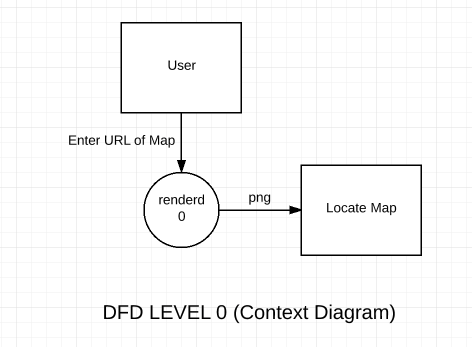
\includegraphics[scale=0.6]{input/images/DFD_0.png}
\caption{Data Flow Diagram Level 0}
\end{figure}
\begin{figure}[h!]
	\centering
	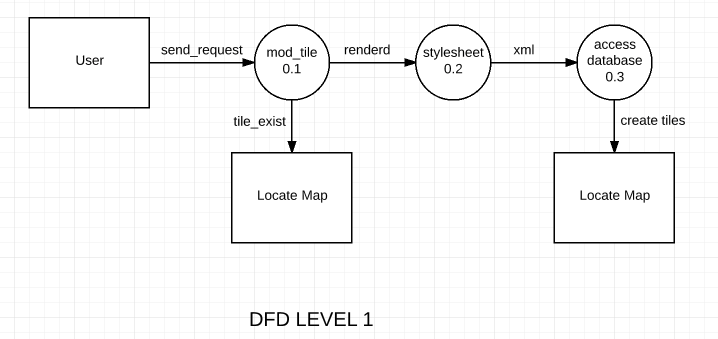
\includegraphics[scale=0.6]{input/images/DFD_1.png}
	\caption{Data Flow Diagram Level 1}
\end{figure}
\begin{figure}[h!]
	\centering
	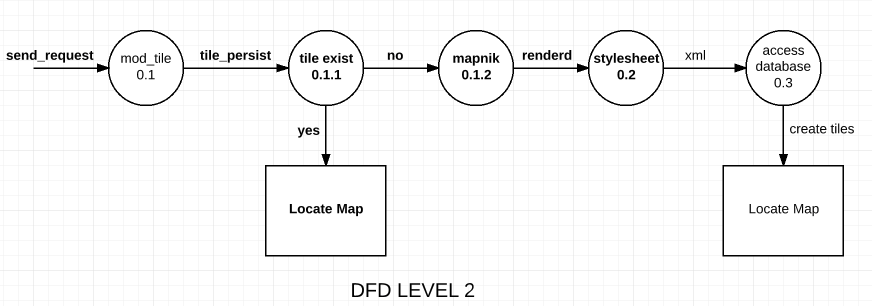
\includegraphics[scale=0.6]{input/images/DFD_2.png}
	\caption{Data Flow Diagram Level 2}
\end{figure}

\section{Flowchart}
A flowchart is a type of diagram that represents an algorithm, work flow or process, showing the steps as boxes of various kinds, and their order by connecting them with arrows
and following are flowchart of showing flow of control and Data in the software-:

\begin{figure}[h!]
	\centering
	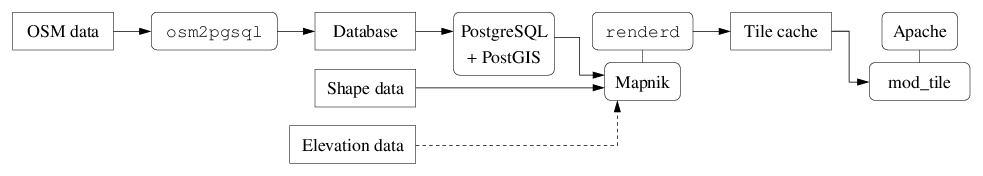
\includegraphics[scale=0.6]{input/images/osmserv.png}
	\caption{Data Flow Of Whole System}
\end{figure}



\begin{figure}[h!]
\centering
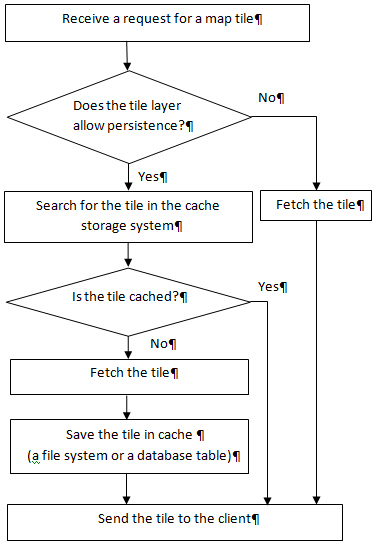
\includegraphics[scale=0.9]{input/images/fetch.jpg}
\caption{Flow Chart to Serve a Tile}
\end{figure}
\hspace{-1.7em}



\section{Problem Formulation}
Geographical data (geo data) is not free in many parts of the world.\\
Because that data is copyrighted and owned by multiple organisations like the Ordnance Survey. Google/whoever just licenses it. If we were to use it, we'd have to pay for it. \\
\noindent "OpenStreetMap is a free editable map of the whole world. It is made by people like you." Which means the database will always be subject to the whims, experimentation, and mistakes of the community. This is precisely OSM's strength since, among other things, it allows our data to quickly accommodate changes in the physical world.\\
\noindent By making your system an OSM tile server not only you can edit the map but can use it offline also. You can change the styling of the map like color of the roads fonts style and amny more as per your requirments. 


\section{Dependencies}
%\subsection{Hardware Requirements}
\begin{itemize}
\item Operating System: Linux/Windows
\item Processor Speed: 512KHz or more
\item RAM: Minimum 2GB
\item Library: Mapnik
\item Modules: Mod\_tile
\item Compiler: CartoCSS
\item Stylesheet: OSMBright
\item Programming Language: C++, Python
\end{itemize}
%\subsection{Software Requirements}
%\begin{itemize}
%\item Library: Mapnik
%\item Modules: Mod\_tile
%\item Compiler: CartoCSS
%\item Stylesheet: OSMBright 
%\item Programming Language: C++, Python 
%\end{itemize}

\section{Methodology}
\begin{itemize}
\item Studying various methods available to solve different problems of numerical analysis.
\item Deciding various input and output parameters of methods.
\item Making the approach modular 
\item Styling the map.
\item Generating documentation
\end{itemize}

\section{Project Work} 
\textbf{Studied Previous System:}\\
Before starting the project, \\\\
\textbf{Learn Linux:}\\
Before starting with project, we have to install various things to make our system an OSM server. So, for that you should know terminal commands because I gonna explain it for Ubuntu only. It is possible on other OS also but you have to work it own. I have provided some basic command also for Linux. \\\\
\textbf{Learn Postgresql:}\\
 We have to go through the basics of postgresql(database) also, such that there
should not be any problem proceeding with project.\\\\
\textbf{Make or Cmake}\\
The softwares like mapnik, mod\_tile, osm2pqsql, are compiled through the Cmake which is basically language. So, we should the basics of it.
\\\\
\textbf{Languages:}\\
We should the basics of the languages like C++, javascript, python etc for manuplating the stylying and rendering of the map.\\\\
\textbf{Input:}\\
Input values are taken from user or default values defined in the file are used.\\\\
\textbf{Output:}\\
According to input values we will get the particular location of the map.


%

\section{Ubuntu: An open source OS}
\begin{figure}[!ht]
\centering

\includegraphics[width=0.3\textwidth]{input/images/ubu.png}
\caption{Ubuntu}
\hspace{-1.5em}
\end{figure}

During my training, I also got familiar with a great and open source Operating System, Ubuntu. Firstly, it was quite difficult for a regular MS Windows user to port to Ubuntu. I did all of my project work using this vast operating system. 
Ubuntu is a Debian-based Linux operating system, with Unity as its default desktop environment. It is based on free software and named after the Southern African philosophy of ubuntu (literally, "human-ness"), which often is translated as "humanity towards others" or "the belief in a universal bond of sharing that connects all humanity".\\

Ubuntu's goal is to be secure "out-of-the box". By default user's programs run with low privileges and cannot corrupt the operating system or other user's files. For increased security, the sudo tool is used to assign temporary privileges for performing administrative tasks, which allows the root account to remain locked and helps prevent inexperienced users from inadvertently making catastrophic system changes or opening security holes.\\




\begin{figure}[h!]
\centering 
\includegraphics[scale=1]{input/images/doxygen.jpeg}
\caption{Doxygen}
\end{figure}
\noindent Doxygen is a documentation generator, a tool for writing software reference 
documentation. The documentation is written within code, and is thus 
relatively easy to keep up to date. Doxygen can cross reference 
documentation and code, so that the reader of a document can easily 
refer to the actual code.

Doxygen supports multiple programming languages, especially C++, C, 
C\#, Objective-C, Java, Python, IDL, VHDL, Fortran and PHP.[2] Doxygen
 is free software, released under the terms of the GNU General Public 
License.\\

\section{Introduction To Doxygen}
\begin{itemize}
\item Requires very little overhead from the writer of the documentation. 
Plain text will do, Markdown is support, and for more fancy or structured 
output HTML tags and/or some of doxygen's special commands can be used.
\item Cross platform: Works on Windows and many Unix flavors (including 
Linux and Mac OS X).
\item Comes with a GUI frontend (Doxywizard) to ease editing the options 
and run doxygen. The GUI is available on Windows, Linux, and Mac OS X.
\item Automatically generates class and collaboration diagrams in HTML 
(as clickable image maps) and $\mbox{\LaTeX}$ (as Encapsulated PostScript 
images).
\item Allows grouping of entities in modules and creating a hierarchy 
of modules.
\item Doxygen can generate a layout which you can use and edit to change 
the layout of each page.
\item Can cope with large projects easily.
\end{itemize}
\subsection{Installation of Doxygen}
Doxygen can be installed using following commands:\\

\hspace{4pt} \$ git clone https://github.com/doxygen/doxygen.git

\hspace{4pt} \$ cd doxygen

\hspace{4pt} \$ ./configure

\hspace{4pt} \$ make

Documentation of this project.

\begin{figure}[h!]
	\centering 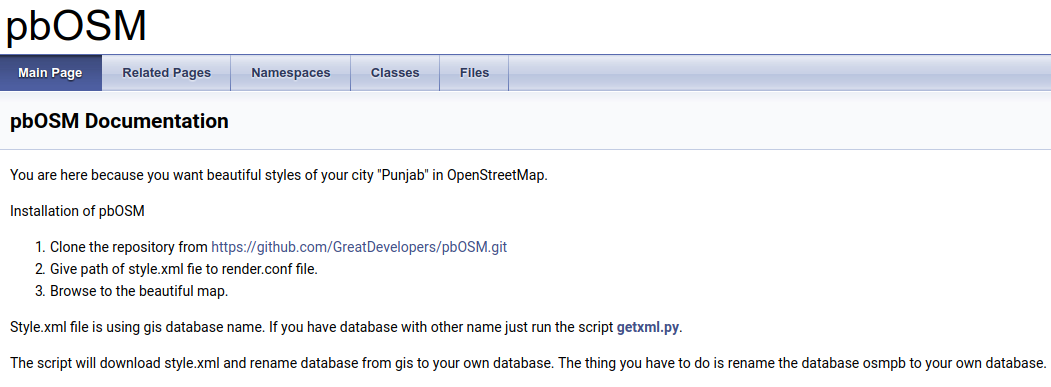
\includegraphics[scale=.4]{input/images/osm_doxygen.png}
	\caption{Main Page of pbOSM}
\end{figure}

\begin{figure}[h!]
	\centering 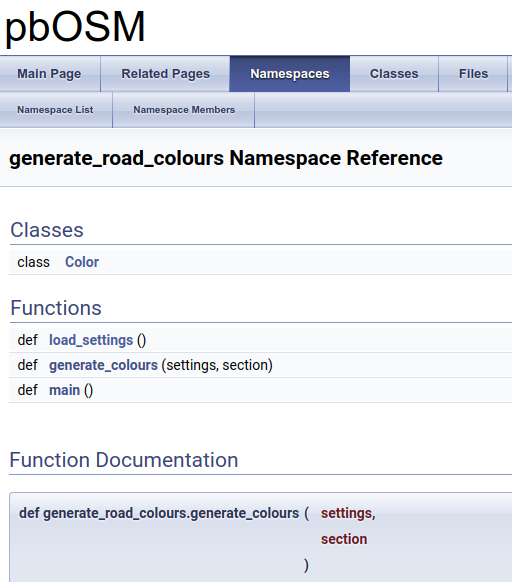
\includegraphics[scale=.6]{input/images/osm_doxygen1.png}
	\caption{Namespace documentation of pbOSM}
\end{figure}




\section{Introduction to \LaTeX}

\LaTeX, I had never heard about this term before doing this project,
but when I came to know about it's features, found it excellent. 
\LaTeX{ is a document markup language and document preparation system for the \TeX{} 
typesetting program. Within the typesetting system, its name is styled 
as \LaTeX.

\begin{figure}[!ht]
\centering
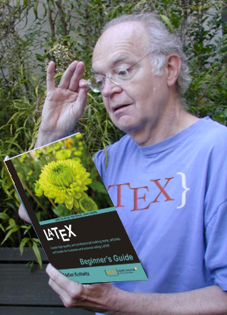
\includegraphics[width=0.3\textwidth]{input/images/donald.png}                   
\caption{Donald Knuth, Inventor Of \TeX{} 
typesetting system}
\hspace{-1.5em}
\end{figure}

Within the typesetting system, its name is styled as \LaTeX. The term 
\LaTeX{} refers only to the language in which documents are written, 
not to the editor used to write those documents. In order to create a 
document in \LaTeX, a .tex file must be created using some form of text 
editor. While most text editors can be used to create a \LaTeX{} document, 
a number of editors have been created specifically for working with \LaTeX.

\LaTeX{} is most widely used by mathematicians, scientists, 
engineers, philosophers, linguists, economists and other scholars in 
academia. As a primary or intermediate format, e.g., translating DocBook 
and other XML-based formats to PDF, \LaTeX{} is used because of the 
high quality of typesetting achievable by \TeX. The typesetting system 
offers programmable desktop publishing features and extensive facilities 
for automating most aspects of typesetting and desktop publishing, 
including numbering and cross-referencing, tables and figures, 
page layout and bibliographies.

\LaTeX{} is intended to provide a high-level language that
accesses the power of \TeX. \LaTeX{} essentially comprises a
collection of \TeX{} macros and a program to process \LaTeX documents. 
Because the \TeX{} formatting commands are very low-level, it is usually 
much simpler for end-users to use \LaTeX{}.


\subsection{Typesetting}
In preparing a \LaTeX{} document, the author 
specifies the logical structure using familiar concepts such as 
chapter, section, table, figure, etc., and lets the \LaTeX{} system 
worry about the presentation of these structures. It therefore 
encourages the separation of layout from content while still allowing 
manual typesetting adjustments where needed. 

\begin{verbatim}
\documentclass[12pt]{article}
\usepackage{amsmath}
\title{\LaTeX}
\date{}
\begin{document}
  \maketitle 
  \LaTeX{} is a document preparation system 
  for the \TeX{} typesetting program.
\end{document}
\end{verbatim}

\begin{figure}[!ht]
\centering
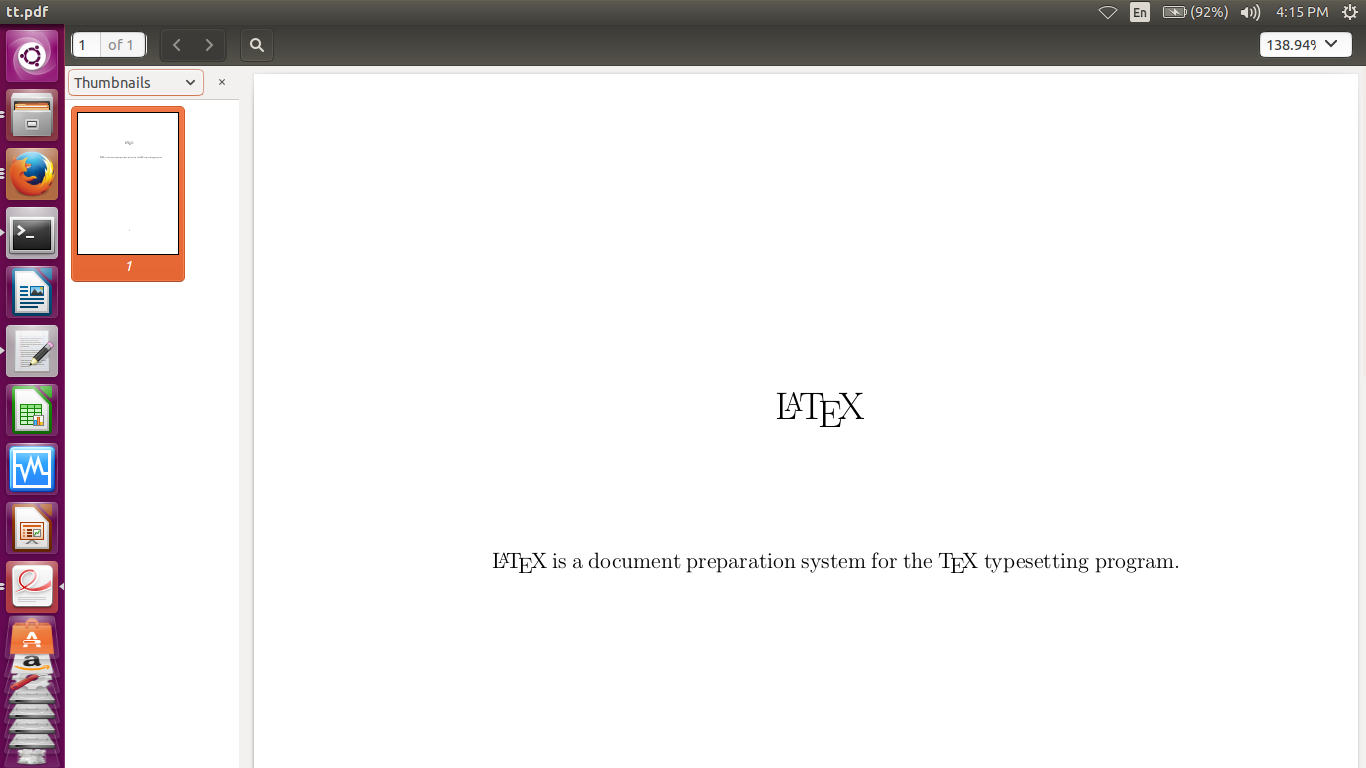
\includegraphics[width=0.5\textwidth]{input/images/la.png}
\caption{Output of the avove program}
\hspace{-1.5em}
\end{figure}


\section{Introduction to Github}
\begin{figure}[!ht]
\centering

\includegraphics[width=0.3\textwidth]{/home/amisha/gitt/6-weeks-report/input/images/github.jpg}                   
\caption{Github Logo}
\hspace{-1.5em}
\end{figure}
\leavevmode\\
GitHub is a Git repository web-based hosting service which offers all of the functionality of Git as well as adding many of its own features. Unlike Git which is strictly a command-line tool, Github provides a web-based graphical interface and desktop as well as mobile integration. It also provides access control and several collaboration features such as wikis, task management, and bug tracking and feature requests for every project.\\

GitHub offers both paid plans for private repo handle everything from small to very large projects with speed and efficiency. ositories, and free accounts, which are usually used to host open source software projects. As of 2014, Github reports having over 3.4 million users, making it the largest code host in the world.\\

GitHub has become such a staple amongst the open-source development community that many developers have begun considering it a replacement for a conventional resume and some employers require applications to provide a link to and have an active contributing GitHub account in order to qualify for a job.\\

The Git feature that really makes it stand apart from nearly every
other Source Code Management (SCM) out there is its branching model.\\
\\
Git allows and encourages you to have multiple local branches that can
be entirely independent of each other. The creation, merging, and
deletion of those lines of development takes seconds.\\ \\
This means that you can do things like:
\begin{itemize}
\item Frictionless Context Switching.\\ Create a branch to try out an
idea, commit a few times, switch back to where you branched from,
apply a patch, switch back to where you are experimenting, and merge
it in.
\item Role-Based Code lines. \\ Have a branch that always contains only
what goes to production, another that you merge work into for testing,
and several smaller ones for day to day work.
\item Feature Based Work flow. \\ Create new branches for each new
feature you're working on so you can seamlessly switch back and forth
between them, then delete each branch when that feature gets merged
into your main line.
\item Disposable Experimentation.\\  Create a branch to experiment in,
realize it's not going to work, and just delete it - abandoning the
work—with nobody else ever seeing it (even if you've pushed other
branches in the meantime).
\end{itemize}
Notably, when you push to a remote repository, you do not have to push
all of your branches. You can choose to share just one of your
branches, a few of them, or all of them. This tends to free people to
try new ideas without worrying about having to plan how and when they
are going to merge it in or share it with others.\\ \\
There are ways to accomplish some of this with other systems, but the
work involved is much more difficult and error-prone. Git makes this
process incredibly easy and it changes the way most developers work
when they learn it.

\subsection{What is Git?}
\begin{figure}[!ht]
\centering

\includegraphics[width=0.3\textwidth]{/home/amisha/gitt/6-weeks-report/input/images/git.jpg}                   
\caption{Git Logo}
\hspace{-1.5em}
\end{figure}
Git is a distributed revision control and source code management (SCM) system with an emphasis on speed, data integrity, and support for distributed, non-linear workflows. Git was initially designed and developed by Linus Torvalds for Linux kernel development in 2005, and has since become the most widely adopted version control system for software development.\\

As with most other distributed revision control systems, and unlike most client–server systems, every Git working directory is a full-fledged repository with complete history and full version-tracking capabilities, independent of network access or a central server. Like the Linux kernel, Git is free and open source software distributed under the terms of the GNU General Public License version 2 to handle everything from small to very large projects with speed and efficiency.\\

Git is easy to learn and has a tiny footprint with lightning fast performance. It outclasses SCM tools like Subversion, CVS, Perforce, and ClearCase with features like cheap local branching, convenient staging areas, and multiple workflows.\\

\subsection{Installation of Git}

Installation of git is a very easy process.
The current git version is: 2.0.4.
Type the commands in the terminal:\\\\
\emph{
\$ sudo apt-get update\\\\
\$ sudo apt-get install git\\\\}
This will install the git on your pc or laptop.

\subsection{Various Git Commands}

Git is the open source distributed version control system that facilitates GitHub activities on your laptop or desktop. The commonly used Git command line instructions are:-\\

\subsubsection{Create Repositories}
Start a new repository or obtain from an exiting URL

\begin{description}

\item [\$ git init [ project-name]]\\
Creates a new local repository with the specified name
\item [\$ git clone [url]]\\
Downloads a project and its entire version history\\

\end{description}


\subsubsection{Make Changes}
Review edits and craft a commit transaction

\begin{description}

\item [\$ git status] \leavevmode \\
Lists all new or modified files to be committed

\item [\$ git diff] \leavevmode \\
Shows file differences not yet staged

\item [\$ git add [file]]\\
Snapshots the file in preparation for versioning

\item [\$ git commit -m "[descriptive message]"]\\
Records file snapshots permanently in version history\\

\end{description}


\subsubsection{Group Changes}
Name a series of commits and combine completed efforts

\begin{description}

\item [\$ git branch] \leavevmode \\
Lists all local branches in the current repository

\item [\$ git branch [branch-name]]\\
Creates a new branch

\item [\$ git checkout [branch-name]]\\
Switches to the specified branch and updates the working directory

\item [\$ git branch -d [branch-name]]\\
Deletes the specified branch\\

\end{description}


\subsubsection{Synchronize Changes}
Register a repository bookmark and exchange version history

\begin{description}

\item [\$ git fetch [bookmark]]\\
Downloads all history from the repository bookmark

\item [\$ git merge [bookmark]/[branch]]\\
Combines bookmark’s branch into current local branch

\item [\$ git push [alias][branch]]\\
Uploads all local branch commits to GitHub

\item [\$ git pull] \leavevmode \\
Downloads bookmark history and incorporates changes

\end{description}



\section{Introduction to Reveal-js \& Reveal-md}
\begin{figure}[!ht]
\centering

\includegraphics[width=0.3\textwidth]{input/images/reveal.png}                   
\caption{MD \& JS}
\hspace{-1.5em}
\end{figure}
Reveal-js is one of the framework of Javascript. This can be used for presentations purpose.\\
Now before going to reveal-md lets talk about some fundamental things.\\
What is a Markup language?\\
Markup languages are designed for the processing, definition and presentation of text. The language specifies code for formatting, both the layout and style, within a text file. HTML and Markdown  is an example of a widely known and used markup language.\\
Markdown is a lightweight Markup Language with simple plain text formatting syntax designed so that it can be converted to HTML and many other formats. It is created by  John Gruber. It had '.md' or '.markdown' extention.\\
"Markdown is a text-to-HTML conversion software tool written in Perl for web writers."\\
Moreover, to enable markdown feature of reveal.js, we need reveal-md. The Markdown feature of reveal.js is awesome, and has an easy (and configurable) syntax to separate slides. Use three dashes surrounded by two blank lines.\\
\subsection{Installation of reveal-md}
Installation of reveal-md is a very easy process.
Type the commands in the terminal:\\\\
\emph{
\$ sudo apt-get install npm\\\\
\$ sudo apt-get install nodejs-legacy\\\\
\$ sudo npm install -g reveal-md\\\\}
This will install reveal-md on your pc or laptop.



\section{Working with Experimental Server}
\begin{figure}[!ht]
\centering

\includegraphics[width=0.3\textwidth]{input/images/ser.png}                   
\caption{Server Communication}
\hspace{-1.5em}
\end{figure}
I had also done the whole project on ubuntu experimental server and had also learnt about making your system a server.\\
What is a Remote Server?\\
In simple words its nothing much but a Computer that is not attached to a user’s keyboard but over which he or she has some degree of control (like can see data of that computer, can retrieve or send data etc.)\\
For going deep you need to know about ssh (Secure Shell). I had  written about it in my old blogs. You can Google it too.\\
I had done it using SSH. There are few terms related to this :\\
\begin{itemize}
\item SSH: It is a Secure Socket Shell, is a network protocol that provides administrators with a secure way to access a remote computer.
\item MOSH: It is a software tool used to connect from a client computer to a server over the Internet, to run a remote terminal. 
\item Tmux: tmux is basically a terminal multiplexer. It is used so that within
one terminal window we can open multiple windows and split-views.
\item OpenSSH: It is a freely available version of the Secure Shell (SSH) protocol family of tools for remotely controlling or transferring files between computers. Traditional tools used to accomplish this is telnet which is not much secure.
\end{itemize}

In Unix, you can use SCP (the scp command) to securely copy files and directories between remote hosts without starting an FTP session or logging into the remote systems explicitly. \\
The scp command uses SSH to transfer data, so it requires a password.\\\\
Some of the useful commands in this for checking errors or for other purposes are: \\
\begin{itemize}
\item ll: This command is used to list the detail information of files and folder of a current directory. 
\item tail -f error.log: This is used for checking errors.
\item sudo apt-get install openssh-server
\item sudo vim /etc/ssh/sshdconfig \\
(To edit this as per your preferences. But first take a backup of this file for later default configurations if needed.)
\item sudo restart ssh \\
(To check your ssh daemon is running or not.)

\item ssh user@hostip \\
(To enter into a remote server from some other system. )
\end{itemize}

 

%\section{Certificate Genertion System}

Apart from the major project i.e OSM I have done another project "Certificate Generation System".

Certificate Generation System is a portable application used to Generate Certificate for single candidate providing his/her details along with image,
As well as for Batch/Number of candidates by simply providing the CSV format file (containing details of every candidate) along with candidate images.

CSV(Character Separated File) is a simple file format used to store tabular data, such as a spreadsheet or database. Files in the CSV format can be imported to and exported from programs that store data in tables, such as Microsoft Excel or OpenOffice Calc.

INSTALLATION/SETUP

This application is a portable application used to Generate Certificate for single candidate providing his/her details along with image,
As well as for Batch/Number of candidates by simply providing the CSV format file (containing details of every candidate) along with candidate images in a compressed (tar.gz or zip) folder.
Requirements(automatically installed during setup)

    Apache web server
    php interpreter
    unoconv
    python3-uno

USER MANUAL

As the Name "Certificate Generation System" Implies this application is used to generate certificate in an automated manner in few steps:

    Select Design from the images shown on the first page. ( Put mouse pointer over the image to see larger view. )

\begin{figure}[!ht]
\centering
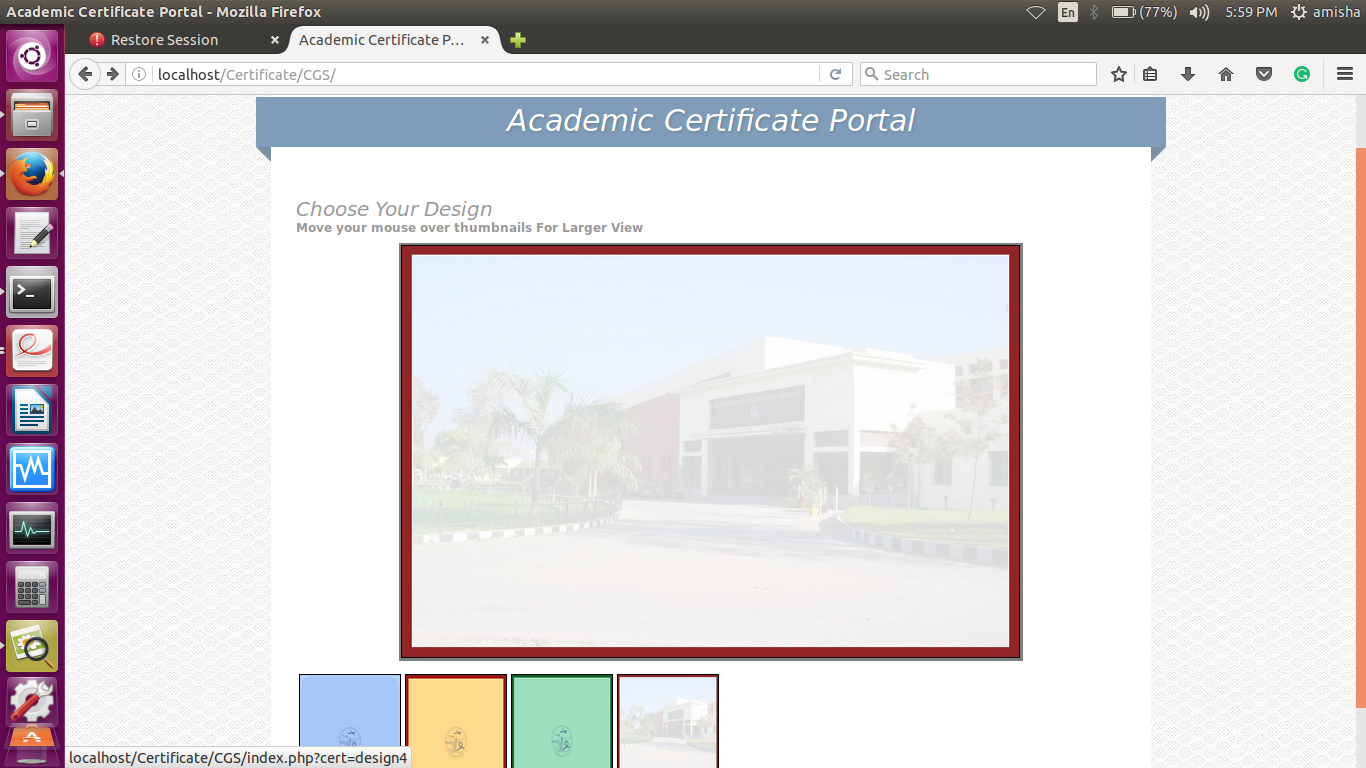
\includegraphics[width=0.7\textwidth]{input/images/cgs/cgs1.png}
\caption{Academic Portal}
\hspace{-1.5em}
\end{figure}


    Next Page will be page for entering Institute Details.


    Fill in the details of institution for which the certificate(s) is to be made.

    Place mouse pointer over Input box te see an example for that input.
\begin{figure}[!ht]
\centering
\includegraphics[width=0.7\textwidth]{input/images/cgs/cgs2.png}                  
\caption{Institute Details}
\hspace{-1.5em}
\end{figure}


    Next page will show two options

    Manual Entry -> Select it for Generating Certificate for Single candidate.

    Upload Csv File -> Select it for Generating certificate for more than 1 candidate by providing their details in Csv file.
    Manual Entry
\begin{figure}[!ht]
\centering
\includegraphics[width=0.7\textwidth]{input/images/cgs/cgs3.png}                  
\caption{Select Manual Option}
\hspace{-1.5em}
\end{figure}

    On Selecting Manual Entry Next page will open containing input boxes for candidate Details.

    Enter the details and select the image also.

    Live Image Selector

    Next you will be displayed your selected image and a selection box.

\begin{figure}[!ht]
\centering
\includegraphics[width=0.7\textwidth]{input/images/cgs/cgs4.png}                  
\caption{Candidate Details Form}
\hspace{-1.5em}
\end{figure}

    Resize and move the selection box to desired position and size.

\begin{figure}[!ht]
\centering
\includegraphics[width=0.7\textwidth]{input/images/cgs/cgs5.png}                  
\caption{Crop Image}
\hspace{-1.5em}
\end{figure}

    Download

    Thats it your certificate is generated and can be downloaded in two formats

    -> odt ('O'penOffice 'D'ocument 'T'ext)

    -> pdf ('P'ortable 'D'ocument 'F'ormat)

\begin{figure}[!ht]
\centering
\includegraphics[width=0.7\textwidth]{input/images/cgs/cgs6.png}                  
\caption{Download Certificate}
\hspace{-1.5em}
\end{figure}

\begin{figure}[!ht]
\centering
\includegraphics[width=0.7\textwidth]{input/images/cgs/cgs8.png}                 
\caption{Certificate odt file}
\hspace{-1.5em}
\end{figure}


    Also by clicking on "Generate Another Ceritificate" you can generate another certificate

    with same design & institute details and different Candidate Details.

    And by clicking on "Goto First Page" you can again start from Design Selection Page.
    Upload csv file

    On selecting 'Upload csv File' Next page will open containing the conditions for the files

    to be uploaded for certificate generation.
\begin{figure}[!ht]
\centering
\includegraphics[width=0.7\textwidth]{input/images/cgs/cgs3.png}                  
\caption{Choose csv Option}
\hspace{-1.5em}
\end{figure}
    A sample file can be downloaded from the link provided in the 'Note' in the instructions on page.

    Sample file is a zip file named sample.zip containing the csv file and tar.gz file for images.

    Extract it and then sample certificates can be produced using 'sample.csv' and 'images.tar.gz' files.

\begin{figure}[!ht]
\centering
\includegraphics[width=0.7\textwidth]{input/images/cgs/cgs9.png}                 
\caption{Candidate Details Form}
\hspace{-1.5em}
\end{figure}


    That's it your certificate file is produced for all the candidates provided in the csv data file.

Produced Certificate file can be downloaded in two formats again.

-> odt ('O'penOffice 'D'ocument 'T'ext)

-> pdf ('P'ortable 'D'ocument 'F'ormat)
\begin{figure}[!ht]
\centering
\includegraphics[width=0.7\textwidth]{input/images/cgs/cgs14.png}                  
\caption{Odt file through csv}
\hspace{-1.5em}
\end{figure}

\section{OSM and its Components }
It is a collaborative project to create a free editable map of the world.
Now ,before beginning to make your own tile server, review some termonologies.
\begin{figure}[ht]
\centering \includegraphics[scale=0.6]{input/images/index.jpeg}
\caption{OpenStreetMap logo}
\end{figure}

\subsection{Benifits Of Own Tile Server}
 OSM map is accessible even when internet provider is down or when the power is off or both. It won't take much for to see the benefit of having your own piece of OpenStreetMap infrastructure.\\
Now it's turn to install, setup and configure all the necessary software to operate own tile server. All the instructions are illustrated in blog "https://amisha2016.wordpress.com"\\
These instructions build what OpenStreetMap calls a "tile server". That is, a computer that uses the OSM data set to create map images that are suitable for a website. Not every OpenStreetMap function is supported, but you will be able to create a local map, keep it up to date and customize it for your own purposes.
\begin{figure}[!ht]
\centering
\includegraphics[width=0.4\textwidth]{input/images/index.png}                   
\caption{Postgresql}
\hspace{-1.5em}
\end{figure}


\subsection{Postgresql / postgis}
PostGIS is a spatial database extender for PostgreSQL object-relational database. It adds support for geographic objects allowing location queries to be run in SQL.\\
Most spatial databases allow representing simple geometric objects such as points, lines and polygons. Some spatial databases handle more complex structures such as 3D objects, topological coverages, linear networks, and TINs.\\
On Ubuntu there are pre-packaged versions of both postgis and postgresql, so these can simply be installed via the Ubuntu package manager.\\
\subsection{Osm2pgsql}
 osm2pgsql is under active development and is best compiled from source.\\
osm2pgsql is a command-line based program that converts OpenStreetMap data to postGIS-enabled PostgreSQL databases.\\
Mapnik is an open source mapping toolkit for desktop- and server-based map rendering, written in C++.\\
One of its many users is the OpenStreetMap project (OSM), which uses it in combination with an Apache Web Server module (mod\_tile) to render tiles that make up the OSM ‘Slippy Map’ Layer.\\
\begin{figure}[!ht]
\centering
\includegraphics[width=0.7\textwidth]{input/images/bright.jpeg}                   
\caption{Openstreetmap-carto Style}
\hspace{-1.5em}
\end{figure}



\subsection{Openstreetmap-carto}
Openstreetmap-carto is a sensible starting point for quickly making beautiful maps based on an OpenStreetMap database. It is written in the Carto styling language and can be opened as a project in TileMill.\\
The style is still a work in progress and you are encouraged to use the issue tracker to note missing features or problems with the current implementation.\\
\subsection{OpenLayer.js}
OpenLayers makes it easy to put a dynamic map in any web page. It can display map tiles, vector data and markers loaded from any source. OpenLayers has been developed to further the use of geographic information of all kinds. It is completely free.\\
\subsection{Geographic Information Systems (GIS)}
GIS is a computer system for capturing, storing, checking, and displaying data related to positions on Earth’s surface. GIS can show many different kinds of data on one map. This enables people to more easily see, analyze, and understand patterns and relationships\\
The Global Positioning System (GPS) is a space-based navigation system that provides location and time information in all weather conditions, anywhere on or near the Earth where there is an unobstructed line of sight to four or more GPS satellites.\\


\chapter{Project Design}
\section{Software Requirement Analysis}

Software requirement analysis is a process of gathering and interpreting facts, diagnosing problems and the information to recommend improvements on the system. It is a problem solving activity that requires intensive communication between the system users and system developers. System analysis or study is an important phase of any system development process. The system is studied to the minutest detail and analyzed. The system analyst plays the role of the interrogator and dwells deep into the working of the present system. The system is viewed as a whole and the input to the system are identified. The outputs from the organizations are traced to the various processes. System analysis is concerned with becoming aware of the problem, identifying the relevant and decisional variables, analyzing and synthesizing the various factors and determining an optimal or at least a satisfactory solution or program of action.\\\\

\noindent A detailed study of the process must be made by various techniques like interviews, questionnaires etc. The data collected by these sources must be scrutinized to arrive to a conclusion. The conclusion is an understanding of how the system functions. This system is called the existing system. Now the existing system is subjected to close study and problem areas are identified. The designer now functions as a problem solver and tries to sort out the difficulties that the enterprise faces. The solutions are given as proposals. The proposal is then weighed with the existing system analytically and the best one is selected. The proposal is presented to the user for an endorsement by the user. The proposal is reviewed on user request and suitable changes are made. This is loop that ends as soon as the user is satisfied with proposal.\\\\

\noindent Preliminary study is the process of gathering and interpreting facts, using the information for further studies on the system. Preliminary study is problem solving activity that requires intensive communication between the system users and system developers. It does various feasibility studies. In these studies a rough figure of the system activities can be obtained, from which the decision about the strategies to be followed for effective system study and analysis can be taken.


%\section{Other Specifications}

A Software Requirements Analysis for a software system is a complete 
description of the behavior of a system to be developed. It include functional Requirements
and Software Requirements. In addition to these, the SRS contains 
non-functional requirements. Non-functional requirements are 
requirements which impose constraints on the design or implementation.
\begin{itemize}
\item{\bf Purpose}: OpenStreetMap (OSM) is an open collaborative project to  create a free editable map of the world and the main purpose of this project is to:
\begin{enumerate}
\item  To  create a free editable map of the world.
\item To gather location data  using GPS, local knowledge, and other free sources of information and upload it.
\item  To encourage the growth, development and distribution of free geospatial data. 
\item  To provide geospatial data for anyone to use and share.
\item Reduce the time for analysis.
\item The OpenStreetMap Foundation is an international not-for-profit organization supporting, but not controlling, the OpenStreetMap Project.
\end{enumerate}

\item{\bf Users of the System}
\begin{enumerate} 
\item Client : Clients are the end users that benefit from this project.
They just provide input(like entering name of the area) and gets output(in the form of map).
\begin{enumerate}
\item Researcher or student-: They have knowledge of working of procedures and can edt the map according to their needs.  
\end{enumerate}
\end{enumerate}
\end{itemize}

\subsection{Functional Requirements}
\begin{itemize}
\item {\bf Specific Requirements}: This phase covers the whole requirements 
for the system. After understanding the system we need the input data 
to the system then we watch the output and determine whether the output 
from the system is according to our requirements or not. So what we have 
to input and then what we'll get as output is given in this phase. This 
phase also describe the software and non-function requirements of the 
system.
\item {\bf Input Requirements of the System}
\begin{enumerate} 
\item Guess points and name of the places.
\item Precision
\item Required point at which value is to be found
\item Knowledge of latitude and longitude.
\end{enumerate}
\vskip 0.5cm
\item {\bf Output Requirements of the System}
\begin{enumerate} 
\item Final output of the location of the particulaar area.
\item Shops, restaurants and many more are represented through icon and images.
\end{enumerate}
\vskip 0.5cm
\item {\bf Special User Requirements}
\begin{enumerate} 
\item Taking bulk input values through html forms.
\end{enumerate}
\vskip 0.5cm
\item {\bf Software Requirements}
\begin{enumerate} 
\item Programming language: C++, Python
\item software: \LaTeX{}
\item Web Languages: php, javascript, html
\item Database: Postgresql 
\item Documentation: Doxygen 1.8.3
\item Text Editor: Vim
\item Operating System: Ubuntu 14.04 or 15.10
\item Revision System: Git

\end{enumerate}
\vskip 0.5cm
\subsection{Non functional requirements}
\begin{enumerate} 
\item Scalability: System should be able to handle a number of users. 
For e.g., handling around thousand users at the same time.
\item Usability: Simple user interfaces that a layman can understand.
\item Speed: Processing input should be done in reasonable time
 i.e. we can say maximum 24 hrs.
\end{enumerate}
\end{itemize}



\section{DFDs}
A data flow diagram (DFD) is a graphical representation of the "flow" of data through an information system, modeling its process aspects. A DFD is often used as a preliminary step to create an overview of the system, which can later be elaborated. DFDs to serve a tile is as following-:
\begin{figure}[h!]
\centering
\includegraphics[scale=0.6]{input/images/DFD_0.png}
\caption{Data Flow Diagram Level 0}
\end{figure}
\begin{figure}[h!]
	\centering
	\includegraphics[scale=0.6]{input/images/DFD_1.png}
	\caption{Data Flow Diagram Level 1}
\end{figure}
\begin{figure}[h!]
	\centering
	\includegraphics[scale=0.6]{input/images/DFD_2.png}
	\caption{Data Flow Diagram Level 2}
\end{figure}

\section{Flowchart}
A flowchart is a type of diagram that represents an algorithm, work flow or process, showing the steps as boxes of various kinds, and their order by connecting them with arrows
and following are flowchart of showing flow of control and Data in the software-:

\begin{figure}[h!]
	\centering
	\includegraphics[scale=0.6]{input/images/osmserv.png}
	\caption{Data Flow Of Whole System}
\end{figure}



\begin{figure}[h!]
\centering
\includegraphics[scale=0.9]{input/images/fetch.jpg}
\caption{Flow Chart to Serve a Tile}
\end{figure}
\hspace{-1.7em}



\section{Problem Formulation}
Geographical data (geo data) is not free in many parts of the world.\\
Because that data is copyrighted and owned by multiple organisations like the Ordnance Survey. Google/whoever just licenses it. If we were to use it, we'd have to pay for it. \\
\noindent "OpenStreetMap is a free editable map of the whole world. It is made by people like you." Which means the database will always be subject to the whims, experimentation, and mistakes of the community. This is precisely OSM's strength since, among other things, it allows our data to quickly accommodate changes in the physical world.\\
\noindent By making your system an OSM tile server not only you can edit the map but can use it offline also. You can change the styling of the map like color of the roads fonts style and amny more as per your requirments. 


\section{Dependencies}
%\subsection{Hardware Requirements}
\begin{itemize}
\item Operating System: Linux/Windows
\item Processor Speed: 512KHz or more
\item RAM: Minimum 2GB
\item Library: Mapnik
\item Modules: Mod\_tile
\item Compiler: CartoCSS
\item Stylesheet: OSMBright
\item Programming Language: C++, Python
\end{itemize}
%\subsection{Software Requirements}
%\begin{itemize}
%\item Library: Mapnik
%\item Modules: Mod\_tile
%\item Compiler: CartoCSS
%\item Stylesheet: OSMBright 
%\item Programming Language: C++, Python 
%\end{itemize}

\section{Methodology}
\begin{itemize}
\item Studying various methods available to solve different problems of numerical analysis.
\item Deciding various input and output parameters of methods.
\item Making the approach modular 
\item Styling the map.
\item Generating documentation
\end{itemize}

\section{Project Work} 
\textbf{Studied Previous System:}\\
Before starting the project, \\\\
\textbf{Learn Linux:}\\
Before starting with project, we have to install various things to make our system an OSM server. So, for that you should know terminal commands because I gonna explain it for Ubuntu only. It is possible on other OS also but you have to work it own. I have provided some basic command also for Linux. \\\\
\textbf{Learn Postgresql:}\\
 We have to go through the basics of postgresql(database) also, such that there
should not be any problem proceeding with project.\\\\
\textbf{Make or Cmake}\\
The softwares like mapnik, mod\_tile, osm2pqsql, are compiled through the Cmake which is basically language. So, we should the basics of it.
\\\\
\textbf{Languages:}\\
We should the basics of the languages like C++, javascript, python etc for manuplating the stylying and rendering of the map.\\\\
\textbf{Input:}\\
Input values are taken from user or default values defined in the file are used.\\\\
\textbf{Output:}\\
According to input values we will get the particular location of the map.


%\chapter{Experimental Results and Comparison}
%
\section{Experimental Results}
I had tried my project on different server also i.e Experimental Server here. I had tried it on both ubuntu 14.04 and 15.10. It works fine on both versions.
\begin{figure}[!ht]
	\centering
	\includegraphics[width=0.7\textwidth]{input/images/exp.png}                
	\caption{Graph Plotted}
	\hspace{-1.5em}
\end{figure}\\
You may refer to my blogs also for detailed information.
Here is the url: 
https://amisha2016.wordpress.com/

 
 
 


\chapter{Development and Implementation}
\section[Introduction to Languages]{Introduction to Languages}
Front End languages are language that are used to give better user experince and user interface. These mainly include HTML, CSS, Javascript. Some Frameforks like Bootstrap are also used with these basic languages.
\subsection{HTML}
\begin{figure}[!ht]
\centering
\includegraphics[width=0.3\textwidth]{input/images/HTML.png}                   
\caption{HTML5 Logo}
\hspace{-1.5em}
\end{figure}
HyperText Markup Language, commonly referred to as HTML, is the standard markup language used to create web pages. Along with CSS, and JavaScript, HTML is a cornerstone technology, used by most websites to create visually engaging webpages, user interfaces for web applications, and user interfaces for many mobile applications. Web browsers can read HTML files and render them into visible or audible web pages. HTML describes the structure of a website semantically along with cues for presentation, making it a markup language, rather than a programming language.


HTML elements form the building blocks of all websites. HTML allows images and objects to be embedded and can be used to create interactive forms. It provides a means to create structured documents by denoting structural semantics for text such as headings, paragraphs, lists, links, quotes and other items.

\begin{verbatim}
<!DOCTYPE html>
<html>
  <head>
    <title>This is a title</title>
  </head>
  <body>
    <p>Hello world!</p>
  </body>
</html>

\end{verbatim}


\subsection{CSS}

\begin{figure}[!ht]
\centering
\includegraphics[width=0.3\textwidth]{input/images/CSS.jpg}                   
	\caption{CSS3}
\hspace{-1.5em}
\end{figure}
Cascading Style Sheets (CSS) is a style sheet language used for describing the presentation of a document written in a markup language.Although most often used to set the visual style of web pages and user interfaces written in HTML and XHTML, the language can be applied to any XML document, including plain XML, SVG and XUL, and is applicable to rendering in speech, or on other media. Along with HTML and JavaScript, CSS is a cornerstone technology used by most websites to create visually engaging webpages, user interfaces for web applications, and user interfaces for many mobile applications.


CSS is desgned primarily to enable the separation of document content from document presentation, including aspects such as the layout, colors, and fonts. This separation can improve content accessibility, provide more flexibility and control in the specification of presentation characteristics, enable multiple HTML pages to share formatting by specifying the relevant CSS in a separate .css file, and reduce complexity and repetition in the structural content, such as semantically insignificant tables that were widely used to format pages before consistent CSS rendering was available in all major browsers. CSS makes it possible to separate presentation instructions from the HTML content in a separate file or style section of the HTML file. For each matching HTML element, it provides a list of formatting instructions

\begin{verbatim}
p {
    color: red;
    text-align: center;
} 
\end{verbatim}
\begin{figure}[!ht]
\centering
\includegraphics[width=0.3\textwidth]{input/images/JS.png}
\caption{Javascript}
\hspace{-1.5em}
\end{figure}

JavaScript (/ˈdʒɑːvəˌskrɪpt/) is a high-level, dynamic, untyped, and interpreted programming language. It has been standardized in the ECMAScript language specification. Alongside HTML and CSS, it is one of the three essential technologies of World Wide Web content production; the majority of websites employ it and it is supported by all modern web browsers without plug-ins. JavaScript is prototype-based with first-class functions, making it a multi-paradigm language, supporting object-oriented, imperative, and functional programming styles. It has an API for working with text, arrays, dates and regular expressions, but does not include any I/O, such as networking, storage or graphics facilities, relying for these upon the host environment in which it is embedded.


\begin{figure}[!ht]
	\centering
	\includegraphics[width=0.3\textwidth]{input/images/bootstrap.png}
	\caption{Bootstrap}
	\hspace{-1.5em}
\end{figure}

Bootstrap is a free and open-source collection of tools for creating websites and web applications. It
contains HTML and CSS-based design templates for typography, forms, buttons, navigation and other
interface components, as well as optional JavaScript extensions.\\
It aims to ease the development of dynamic websites and web applications.\\
Bootstrap is a front end framework, that is, an interface for the user, unlike the server-side code which
resides on the "back end" or server.


\iffalse
\subsection{PHP}
\begin{figure}[!ht]
\centering
\includegraphics[width=0.3\textwidth]{input/images/php.png}
\caption{PHP}
\hspace{-1.5em}
\end{figure}
 {\bf What is PHP?}

    PHP is an acronym for "PHP: Hypertext Preprocessor"
    PHP is a widely-used, open source scripting language
    PHP scripts are executed on the server
    PHP is free to download and use

 {\bf What is a PHP File?}

    PHP files can contain text, HTML, CSS, JavaScript, and PHP code
    PHP code are executed on the server, and the result is returned to the browser as plain HTML
    PHP files have extension ".php"

 {\bf What Can PHP Do?}

    PHP can generate dynamic page content
    PHP can create, open, read, write, delete, and close files on the server
    PHP can collect form data
    PHP can send and receive cookies
    PHP can add, delete, modify data in your database
    PHP can be used to control user-access
    PHP can encrypt data

  {\bf Why PHP?}

    PHP runs on various platforms (Windows, Linux, Unix, Mac OS X, etc.)
    PHP is compatible with almost all servers used today (Apache, IIS, etc.)
    PHP supports a wide range of databases
    PHP is free. Download it from the official PHP resource: www.php.net
    PHP is easy to learn and runs efficiently on the server side
\fi
\subsection{CMake}

CMake is a language(for generator of build systems) with abstract build rules and gnu make is a dependency resolves that executes programs. Cmake takes information on how to build programs generates makefiles that build the program. 

Simple Program 

\begin{figure}[!ht]
\centering
\includegraphics[width=0.6\textwidth]{input/images/cgs/hello.png}                   
\caption{test.cpp file}
\hspace{-1.5em}
\end{figure}

\begin{figure}[!ht]
\centering
\includegraphics[width=0.6\textwidth]{input/images/cgs/cm.png}                   
\caption{cmake file}
\hspace{-1.5em}
\end{figure}

\subsection{Shell Scripting}
Normally shells are interactive. It means shell accept command from you (via keyy
board) and execute them. But if you use command one by one (sequence of 'n' numbb
er of commands) , the you can store this sequence of command to text file and tee
ll the shell to execute this text file instead of entering the commands. This iss
 know as shell script.
Shell script defined as series of command written in plain text file. Shell scrii
pt is just like batch file is MS-DOS but have more power than the MS-DOS batch ff
ile.
why to Write Shell Script ?
\begin{enumerate}
\item Shell script can take input from user, file and output them on screen.
\item Useful to create our own commands.
\item Save lots of time.
\item To automate some task of day today life.
\item System Administration part can be also automated.
\end{enumerate}
{ \bf Execute your script as syntax:}
\begin{verbatim}
chmod 755 your-script-name
sh your-script-name
./your-script-name
\end{verbatim}

\subsection{Python}
\begin{figure}[h]
	\centering \includegraphics[scale=0.3]{input/images/python.png}
	\caption{Python logo}
\end{figure}
\noindent Python is a dynamic language, as in python coding is very easy and 
also it require less coding and about its interpreted nature it is 
just exellent. Python is a high level programming language and Django 
which is a web development framework is written in python language.

Python is an easy to learn, powerful programming language.Python runs 
on Windows, Linux/Unix, Mac OS X. Python is free to use, even for 
commercial products. Python can also be used as an extension language 
for existing modules and applications that need a programmable interface.  
Python is free to use, even for commercial products, because of its 
OSI-approved open source license.
\subsection{Features of Python}
\begin{itemize}
	\item Very clear, readable syntax.
	\item Strong introspection capabilities.
	\item Intuitive object orientation.

\end{itemize}




\section{Ubuntu: An open source OS}
\begin{figure}[!ht]
\centering
\includegraphics[width=0.3\textwidth]{input/images/ubu.png}
\caption{Ubuntu}
\hspace{-1.5em}
\end{figure}

During my training, I also got familiar with a great and open source Operating System, Ubuntu. Firstly, it was quite difficult for a regular MS Windows user to port to Ubuntu. I did all of my project work using this vast operating system. 
Ubuntu is a Debian-based Linux operating system, with Unity as its default desktop environment. It is based on free software and named after the Southern African philosophy of ubuntu (literally, "human-ness"), which often is translated as "humanity towards others" or "the belief in a universal bond of sharing that connects all humanity".\\

Ubuntu's goal is to be secure "out-of-the box". By default user's programs run with low privileges and cannot corrupt the operating system or other user's files. For increased security, the sudo tool is used to assign temporary privileges for performing administrative tasks, which allows the root account to remain locked and helps prevent inexperienced users from inadvertently making catastrophic system changes or opening security holes.\\




\begin{figure}[h!]
\centering \includegraphics[scale=1]{input/images/doxygen.jpeg}
\caption{Doxygen}
\end{figure}
\noindent Doxygen is a documentation generator, a tool for writing software reference 
documentation. The documentation is written within code, and is thus 
relatively easy to keep up to date. Doxygen can cross reference 
documentation and code, so that the reader of a document can easily 
refer to the actual code.

Doxygen supports multiple programming languages, especially C++, C, 
C\#, Objective-C, Java, Python, IDL, VHDL, Fortran and PHP.[2] Doxygen
 is free software, released under the terms of the GNU General Public 
License.\\

\section{Introduction To Doxygen}
\begin{itemize}
\item Requires very little overhead from the writer of the documentation. 
Plain text will do, Markdown is support, and for more fancy or structured 
output HTML tags and/or some of doxygen's special commands can be used.
\item Cross platform: Works on Windows and many Unix flavors (including 
Linux and Mac OS X).
\item Comes with a GUI frontend (Doxywizard) to ease editing the options 
and run doxygen. The GUI is available on Windows, Linux, and Mac OS X.
\item Automatically generates class and collaboration diagrams in HTML 
(as clickable image maps) and $\mbox{\LaTeX}$ (as Encapsulated PostScript 
images).
\item Allows grouping of entities in modules and creating a hierarchy 
of modules.
\item Doxygen can generate a layout which you can use and edit to change 
the layout of each page.
\item Can cope with large projects easily.
\end{itemize}
\subsection{Installation of Doxygen}
Doxygen can be installed using following commands:\\

\hspace{4pt} \$ git clone https://github.com/doxygen/doxygen.git

\hspace{4pt} \$ cd doxygen

\hspace{4pt} \$ ./configure

\hspace{4pt} \$ make

Documentation of this project.

\begin{figure}[h!]
	\centering \includegraphics[scale=.4]{input/images/osm_doxygen.png}
	\caption{Main Page of pbOSM}
\end{figure}

\begin{figure}[h!]
	\centering \includegraphics[scale=.6]{input/images/osm_doxygen1.png}
	\caption{Namespace documentation of pbOSM}
\end{figure}




\section{Introduction to \LaTeX}

\LaTeX, I had never heard about this term before doing this project,
but when I came to know about it's features, found it excellent. 
\LaTeX{ is a document markup language and document preparation system for the \TeX{} 
typesetting program. Within the typesetting system, its name is styled 
as \LaTeX.

\begin{figure}[!ht]
\centering
\includegraphics[width=0.3\textwidth]{input/images/donald.png}                   
\caption{Donald Knuth, Inventor Of \TeX{} 
typesetting system}
\hspace{-1.5em}
\end{figure}

Within the typesetting system, its name is styled as \LaTeX. The term 
\LaTeX{} refers only to the language in which documents are written, 
not to the editor used to write those documents. In order to create a 
document in \LaTeX, a .tex file must be created using some form of text 
editor. While most text editors can be used to create a \LaTeX{} document, 
a number of editors have been created specifically for working with \LaTeX.

\LaTeX{} is most widely used by mathematicians, scientists, 
engineers, philosophers, linguists, economists and other scholars in 
academia. As a primary or intermediate format, e.g., translating DocBook 
and other XML-based formats to PDF, \LaTeX{} is used because of the 
high quality of typesetting achievable by \TeX. The typesetting system 
offers programmable desktop publishing features and extensive facilities 
for automating most aspects of typesetting and desktop publishing, 
including numbering and cross-referencing, tables and figures, 
page layout and bibliographies.

\LaTeX{} is intended to provide a high-level language that
accesses the power of \TeX. \LaTeX{} essentially comprises a
collection of \TeX{} macros and a program to process \LaTeX documents. 
Because the \TeX{} formatting commands are very low-level, it is usually 
much simpler for end-users to use \LaTeX{}.


\subsection{Typesetting}
In preparing a \LaTeX{} document, the author 
specifies the logical structure using familiar concepts such as 
chapter, section, table, figure, etc., and lets the \LaTeX{} system 
worry about the presentation of these structures. It therefore 
encourages the separation of layout from content while still allowing 
manual typesetting adjustments where needed. 

\begin{verbatim}
\documentclass[12pt]{article}
\usepackage{amsmath}
\title{\LaTeX}
\date{}
\begin{document}
  \maketitle 
  \LaTeX{} is a document preparation system 
  for the \TeX{} typesetting program.
\end{document}
\end{verbatim}

\begin{figure}[!ht]
\centering
\includegraphics[width=0.5\textwidth]{input/images/la.png}
\caption{Output of the avove program}
\hspace{-1.5em}
\end{figure}


\section{Introduction to Github}
\begin{figure}[!ht]
\centering
\includegraphics[width=0.3\textwidth]{/home/amisha/gitt/6-weeks-report/input/images/github.jpg}                   
\caption{Github Logo}
\hspace{-1.5em}
\end{figure}
\leavevmode\\
GitHub is a Git repository web-based hosting service which offers all of the functionality of Git as well as adding many of its own features. Unlike Git which is strictly a command-line tool, Github provides a web-based graphical interface and desktop as well as mobile integration. It also provides access control and several collaboration features such as wikis, task management, and bug tracking and feature requests for every project.\\

GitHub offers both paid plans for private repo handle everything from small to very large projects with speed and efficiency. ositories, and free accounts, which are usually used to host open source software projects. As of 2014, Github reports having over 3.4 million users, making it the largest code host in the world.\\

GitHub has become such a staple amongst the open-source development community that many developers have begun considering it a replacement for a conventional resume and some employers require applications to provide a link to and have an active contributing GitHub account in order to qualify for a job.\\

The Git feature that really makes it stand apart from nearly every
other Source Code Management (SCM) out there is its branching model.\\
\\
Git allows and encourages you to have multiple local branches that can
be entirely independent of each other. The creation, merging, and
deletion of those lines of development takes seconds.\\ \\
This means that you can do things like:
\begin{itemize}
\item Frictionless Context Switching.\\ Create a branch to try out an
idea, commit a few times, switch back to where you branched from,
apply a patch, switch back to where you are experimenting, and merge
it in.
\item Role-Based Code lines. \\ Have a branch that always contains only
what goes to production, another that you merge work into for testing,
and several smaller ones for day to day work.
\item Feature Based Work flow. \\ Create new branches for each new
feature you're working on so you can seamlessly switch back and forth
between them, then delete each branch when that feature gets merged
into your main line.
\item Disposable Experimentation.\\  Create a branch to experiment in,
realize it's not going to work, and just delete it - abandoning the
work—with nobody else ever seeing it (even if you've pushed other
branches in the meantime).
\end{itemize}
Notably, when you push to a remote repository, you do not have to push
all of your branches. You can choose to share just one of your
branches, a few of them, or all of them. This tends to free people to
try new ideas without worrying about having to plan how and when they
are going to merge it in or share it with others.\\ \\
There are ways to accomplish some of this with other systems, but the
work involved is much more difficult and error-prone. Git makes this
process incredibly easy and it changes the way most developers work
when they learn it.

\subsection{What is Git?}
\begin{figure}[!ht]
\centering
\includegraphics[width=0.3\textwidth]{/home/amisha/gitt/6-weeks-report/input/images/git.jpg}                   
\caption{Git Logo}
\hspace{-1.5em}
\end{figure}
Git is a distributed revision control and source code management (SCM) system with an emphasis on speed, data integrity, and support for distributed, non-linear workflows. Git was initially designed and developed by Linus Torvalds for Linux kernel development in 2005, and has since become the most widely adopted version control system for software development.\\

As with most other distributed revision control systems, and unlike most client–server systems, every Git working directory is a full-fledged repository with complete history and full version-tracking capabilities, independent of network access or a central server. Like the Linux kernel, Git is free and open source software distributed under the terms of the GNU General Public License version 2 to handle everything from small to very large projects with speed and efficiency.\\

Git is easy to learn and has a tiny footprint with lightning fast performance. It outclasses SCM tools like Subversion, CVS, Perforce, and ClearCase with features like cheap local branching, convenient staging areas, and multiple workflows.\\

\subsection{Installation of Git}

Installation of git is a very easy process.
The current git version is: 2.0.4.
Type the commands in the terminal:\\\\
\emph{
\$ sudo apt-get update\\\\
\$ sudo apt-get install git\\\\}
This will install the git on your pc or laptop.

\subsection{Various Git Commands}

Git is the open source distributed version control system that facilitates GitHub activities on your laptop or desktop. The commonly used Git command line instructions are:-\\

\subsubsection{Create Repositories}
Start a new repository or obtain from an exiting URL

\begin{description}

\item [\$ git init [ project-name]]\\
Creates a new local repository with the specified name
\item [\$ git clone [url]]\\
Downloads a project and its entire version history\\

\end{description}


\subsubsection{Make Changes}
Review edits and craft a commit transaction

\begin{description}

\item [\$ git status] \leavevmode \\
Lists all new or modified files to be committed

\item [\$ git diff] \leavevmode \\
Shows file differences not yet staged

\item [\$ git add [file]]\\
Snapshots the file in preparation for versioning

\item [\$ git commit -m "[descriptive message]"]\\
Records file snapshots permanently in version history\\

\end{description}


\subsubsection{Group Changes}
Name a series of commits and combine completed efforts

\begin{description}

\item [\$ git branch] \leavevmode \\
Lists all local branches in the current repository

\item [\$ git branch [branch-name]]\\
Creates a new branch

\item [\$ git checkout [branch-name]]\\
Switches to the specified branch and updates the working directory

\item [\$ git branch -d [branch-name]]\\
Deletes the specified branch\\

\end{description}


\subsubsection{Synchronize Changes}
Register a repository bookmark and exchange version history

\begin{description}

\item [\$ git fetch [bookmark]]\\
Downloads all history from the repository bookmark

\item [\$ git merge [bookmark]/[branch]]\\
Combines bookmark’s branch into current local branch

\item [\$ git push [alias][branch]]\\
Uploads all local branch commits to GitHub

\item [\$ git pull] \leavevmode \\
Downloads bookmark history and incorporates changes

\end{description}



\section{Introduction to Reveal-js \& Reveal-md}
\begin{figure}[!ht]
\centering
\includegraphics[width=0.3\textwidth]{input/images/reveal.png}                   
\caption{MD \& JS}
\hspace{-1.5em}
\end{figure}
Reveal-js is one of the framework of Javascript. This can be used for presentations purpose.\\
Now before going to reveal-md lets talk about some fundamental things.\\
What is a Markup language?\\
Markup languages are designed for the processing, definition and presentation of text. The language specifies code for formatting, both the layout and style, within a text file. HTML and Markdown  is an example of a widely known and used markup language.\\
Markdown is a lightweight Markup Language with simple plain text formatting syntax designed so that it can be converted to HTML and many other formats. It is created by  John Gruber. It had '.md' or '.markdown' extention.\\
"Markdown is a text-to-HTML conversion software tool written in Perl for web writers."\\
Moreover, to enable markdown feature of reveal.js, we need reveal-md. The Markdown feature of reveal.js is awesome, and has an easy (and configurable) syntax to separate slides. Use three dashes surrounded by two blank lines.\\
\subsection{Installation of reveal-md}
Installation of reveal-md is a very easy process.
Type the commands in the terminal:\\\\
\emph{
\$ sudo apt-get install npm\\\\
\$ sudo apt-get install nodejs-legacy\\\\
\$ sudo npm install -g reveal-md\\\\}
This will install reveal-md on your pc or laptop.



\section{Working with Experimental Server}
\begin{figure}[!ht]
\centering
\includegraphics[width=0.3\textwidth]{input/images/ser.png}                   
\caption{Server Communication}
\hspace{-1.5em}
\end{figure}
I had also done the whole project on ubuntu experimental server and had also learnt about making your system a server.\\
What is a Remote Server?\\
In simple words its nothing much but a Computer that is not attached to a user’s keyboard but over which he or she has some degree of control (like can see data of that computer, can retrieve or send data etc.)\\
For going deep you need to know about ssh (Secure Shell). I had  written about it in my old blogs. You can Google it too.\\
I had done it using SSH. There are few terms related to this :\\
\begin{itemize}
\item SSH: It is a Secure Socket Shell, is a network protocol that provides administrators with a secure way to access a remote computer.
\item MOSH: It is a software tool used to connect from a client computer to a server over the Internet, to run a remote terminal. 
\item Tmux: tmux is basically a terminal multiplexer. It is used so that within
one terminal window we can open multiple windows and split-views.
\item OpenSSH: It is a freely available version of the Secure Shell (SSH) protocol family of tools for remotely controlling or transferring files between computers. Traditional tools used to accomplish this is telnet which is not much secure.
\end{itemize}

In Unix, you can use SCP (the scp command) to securely copy files and directories between remote hosts without starting an FTP session or logging into the remote systems explicitly. \\
The scp command uses SSH to transfer data, so it requires a password.\\\\
Some of the useful commands in this for checking errors or for other purposes are: \\
\begin{itemize}
\item ll: This command is used to list the detail information of files and folder of a current directory. 
\item tail -f error.log: This is used for checking errors.
\item sudo apt-get install openssh-server
\item sudo vim /etc/ssh/sshdconfig \\
(To edit this as per your preferences. But first take a backup of this file for later default configurations if needed.)
\item sudo restart ssh \\
(To check your ssh daemon is running or not.)

\item ssh user@hostip \\
(To enter into a remote server from some other system. )
\end{itemize}

 

%\section{Certificate Genertion System}

Apart from the major project i.e OSM I have done another project "Certificate Generation System".

Certificate Generation System is a portable application used to Generate Certificate for single candidate providing his/her details along with image,
As well as for Batch/Number of candidates by simply providing the CSV format file (containing details of every candidate) along with candidate images.

CSV(Character Separated File) is a simple file format used to store tabular data, such as a spreadsheet or database. Files in the CSV format can be imported to and exported from programs that store data in tables, such as Microsoft Excel or OpenOffice Calc.

INSTALLATION/SETUP

This application is a portable application used to Generate Certificate for single candidate providing his/her details along with image,
As well as for Batch/Number of candidates by simply providing the CSV format file (containing details of every candidate) along with candidate images in a compressed (tar.gz or zip) folder.
Requirements(automatically installed during setup)

    Apache web server
    php interpreter
    unoconv
    python3-uno

USER MANUAL

As the Name "Certificate Generation System" Implies this application is used to generate certificate in an automated manner in few steps:

    Select Design from the images shown on the first page. ( Put mouse pointer over the image to see larger view. )

\begin{figure}[!ht]
\centering
\includegraphics[width=0.7\textwidth]{input/images/cgs/cgs1.png}
\caption{Academic Portal}
\hspace{-1.5em}
\end{figure}


    Next Page will be page for entering Institute Details.


    Fill in the details of institution for which the certificate(s) is to be made.

    Place mouse pointer over Input box te see an example for that input.
\begin{figure}[!ht]
\centering
\includegraphics[width=0.7\textwidth]{input/images/cgs/cgs2.png}                  
\caption{Institute Details}
\hspace{-1.5em}
\end{figure}


    Next page will show two options

    Manual Entry -> Select it for Generating Certificate for Single candidate.

    Upload Csv File -> Select it for Generating certificate for more than 1 candidate by providing their details in Csv file.
    Manual Entry
\begin{figure}[!ht]
\centering
\includegraphics[width=0.7\textwidth]{input/images/cgs/cgs3.png}                  
\caption{Select Manual Option}
\hspace{-1.5em}
\end{figure}

    On Selecting Manual Entry Next page will open containing input boxes for candidate Details.

    Enter the details and select the image also.

    Live Image Selector

    Next you will be displayed your selected image and a selection box.

\begin{figure}[!ht]
\centering
\includegraphics[width=0.7\textwidth]{input/images/cgs/cgs4.png}                  
\caption{Candidate Details Form}
\hspace{-1.5em}
\end{figure}

    Resize and move the selection box to desired position and size.

\begin{figure}[!ht]
\centering
\includegraphics[width=0.7\textwidth]{input/images/cgs/cgs5.png}                  
\caption{Crop Image}
\hspace{-1.5em}
\end{figure}

    Download

    Thats it your certificate is generated and can be downloaded in two formats

    -> odt ('O'penOffice 'D'ocument 'T'ext)

    -> pdf ('P'ortable 'D'ocument 'F'ormat)

\begin{figure}[!ht]
\centering
\includegraphics[width=0.7\textwidth]{input/images/cgs/cgs6.png}                  
\caption{Download Certificate}
\hspace{-1.5em}
\end{figure}

\begin{figure}[!ht]
\centering
\includegraphics[width=0.7\textwidth]{input/images/cgs/cgs8.png}                 
\caption{Certificate odt file}
\hspace{-1.5em}
\end{figure}


    Also by clicking on "Generate Another Ceritificate" you can generate another certificate

    with same design & institute details and different Candidate Details.

    And by clicking on "Goto First Page" you can again start from Design Selection Page.
    Upload csv file

    On selecting 'Upload csv File' Next page will open containing the conditions for the files

    to be uploaded for certificate generation.
\begin{figure}[!ht]
\centering
\includegraphics[width=0.7\textwidth]{input/images/cgs/cgs3.png}                  
\caption{Choose csv Option}
\hspace{-1.5em}
\end{figure}
    A sample file can be downloaded from the link provided in the 'Note' in the instructions on page.

    Sample file is a zip file named sample.zip containing the csv file and tar.gz file for images.

    Extract it and then sample certificates can be produced using 'sample.csv' and 'images.tar.gz' files.

\begin{figure}[!ht]
\centering
\includegraphics[width=0.7\textwidth]{input/images/cgs/cgs9.png}                 
\caption{Candidate Details Form}
\hspace{-1.5em}
\end{figure}


    That's it your certificate file is produced for all the candidates provided in the csv data file.

Produced Certificate file can be downloaded in two formats again.

-> odt ('O'penOffice 'D'ocument 'T'ext)

-> pdf ('P'ortable 'D'ocument 'F'ormat)
\begin{figure}[!ht]
\centering
\includegraphics[width=0.7\textwidth]{input/images/cgs/cgs14.png}                  
\caption{Odt file through csv}
\hspace{-1.5em}
\end{figure}

\section{OSM and its Components }
It is a collaborative project to create a free editable map of the world.
Now ,before beginning to make your own tile server, review some termonologies.
\begin{figure}[ht]
\centering \includegraphics[scale=0.6]{input/images/index.jpeg}
\caption{OpenStreetMap logo}
\end{figure}

\subsection{Benifits Of Own Tile Server}
 OSM map is accessible even when internet provider is down or when the power is off or both. It won't take much for to see the benefit of having your own piece of OpenStreetMap infrastructure.\\
Now it's turn to install, setup and configure all the necessary software to operate own tile server. All the instructions are illustrated in blog "https://amisha2016.wordpress.com"\\
These instructions build what OpenStreetMap calls a "tile server". That is, a computer that uses the OSM data set to create map images that are suitable for a website. Not every OpenStreetMap function is supported, but you will be able to create a local map, keep it up to date and customize it for your own purposes.
\begin{figure}[!ht]
\centering
\includegraphics[width=0.4\textwidth]{input/images/index.png}                   
\caption{Postgresql}
\hspace{-1.5em}
\end{figure}


\subsection{Postgresql / postgis}
PostGIS is a spatial database extender for PostgreSQL object-relational database. It adds support for geographic objects allowing location queries to be run in SQL.\\
Most spatial databases allow representing simple geometric objects such as points, lines and polygons. Some spatial databases handle more complex structures such as 3D objects, topological coverages, linear networks, and TINs.\\
On Ubuntu there are pre-packaged versions of both postgis and postgresql, so these can simply be installed via the Ubuntu package manager.\\
\subsection{Osm2pgsql}
 osm2pgsql is under active development and is best compiled from source.\\
osm2pgsql is a command-line based program that converts OpenStreetMap data to postGIS-enabled PostgreSQL databases.\\
Mapnik is an open source mapping toolkit for desktop- and server-based map rendering, written in C++.\\
One of its many users is the OpenStreetMap project (OSM), which uses it in combination with an Apache Web Server module (mod\_tile) to render tiles that make up the OSM ‘Slippy Map’ Layer.\\
\begin{figure}[!ht]
\centering
\includegraphics[width=0.7\textwidth]{input/images/bright.jpeg}                   
\caption{Openstreetmap-carto Style}
\hspace{-1.5em}
\end{figure}



\subsection{Openstreetmap-carto}
Openstreetmap-carto is a sensible starting point for quickly making beautiful maps based on an OpenStreetMap database. It is written in the Carto styling language and can be opened as a project in TileMill.\\
The style is still a work in progress and you are encouraged to use the issue tracker to note missing features or problems with the current implementation.\\
\subsection{OpenLayer.js}
OpenLayers makes it easy to put a dynamic map in any web page. It can display map tiles, vector data and markers loaded from any source. OpenLayers has been developed to further the use of geographic information of all kinds. It is completely free.\\
\subsection{Geographic Information Systems (GIS)}
GIS is a computer system for capturing, storing, checking, and displaying data related to positions on Earth’s surface. GIS can show many different kinds of data on one map. This enables people to more easily see, analyze, and understand patterns and relationships\\
The Global Positioning System (GPS) is a space-based navigation system that provides location and time information in all weather conditions, anywhere on or near the Earth where there is an unobstructed line of sight to four or more GPS satellites.\\


\section{Implementation}
Development of OSM started with development in phases which focus on particular need of project.
Various phases and their detail are given below -:
\begin{itemize}
\item Phase I (Setup OSM Server) -: \\
        During Phase I, install all the dependecies(components) as mentioned above to make your own osm tile sever. After installing the softwares download the map in pbf(may be osm) format and render your own tile server. You can see your map on the browser after moving to the location which is being downloaded.

\begin{figure}[ht]
\centering \includegraphics[width=0.7\textwidth]{/home/amisha/gitt/6-weeks-report/input/images/osm7.png}
\caption{OSM Map on Browser}
\end{figure}

\item Phase II (Styling of Map) -: \\
        During phase II, we change the colors of the buildings, roads, primary lines, secondary lines etc and then rerender the map to view the changes in the map. I have mention which files needs to be change to proceed furthur in my blog.  
\begin{figure}[ht]
\centering \includegraphics[width=0.7\textwidth]{/home/amisha/gitt/6-weeks-report/input/images/osm5.png}
\caption{Map Styling}
\end{figure}

\item Phase III (User Input Map) -: \\
        During phase III, we made the html and php pages in which user can input latitude, longitude and zoom level of his own choice and if the tile image of that location is downloaded then on one click the map of that particular location will be visible. The functioning is done with the help of Javascript.
\begin{figure}[ht]
\centering \includegraphics[width=0.7\textwidth]{/home/amisha/gitt/6-weeks-report/input/images/osm2.png}
\caption{User Input Page}
\end{figure}

\begin{figure}[ht]
\centering \includegraphics[width=0.7\textwidth]{/home/amisha/gitt/6-weeks-report/input/images/osm3.png}
\caption{Php Page}
\end{figure}

\item Phase IV (OSM Script) -: \\
        During phase IV, we made OSM installation and configuration script. It is the shell non- interactive script means user have to change hardly two three parameters inside the script at the initial stage and then can run the script and can go for having a cup of coffee. The whole script is on my github account.
\item Phase V (Event Handling) -: \\
During phase V, we tried to control the movement of the osm map through the arrow keys of keyboard and we achieved it. Again it is done with the help of Javascript with the concept of event handling. Various formulas are being applied and testing have been done while doing it. The code for the same is on the experimental server. Now, the map can be controlled through arrow keys also. Isn't it amazing. 
\item Phase VI (Insert Pop up Menu and Icons) -: \\
During phase VI, we added textfile containing different attributes like lat, lon, icon etc. At a particular location(through lat and lon) an icon in the form of image showing some message(Pop-up menu mostly with the name of shops at that location). The all points can be disable by disabling the layer "My Points". 
\begin{figure}[ht]
\centering \includegraphics[width=0.7\textwidth]{/home/amisha/gitt/6-weeks-report/input/images/osm1.png}
\caption{Map with pop-up menu and icons}
\end{figure}
\item Phase VII (Map On Remote Server) -: \\
During phase VII, we have added all the things above in the experimental account. It is done so that everyone can see it and for back up purpose also so that the code and project retains on other system also.
\begin{figure}[ht]
\centering \includegraphics[width=0.7\textwidth]{/home/amisha/gitt/6-weeks-report/input/images/osm8.png}
\caption{Map on remote server}
\end{figure}
\item Phase VI (Documentation) -: \\
During final phase, we documented the project( developers documentation and README.md)
using doxygen and wrote the report for this software.
\end{itemize}

\section{Testing}


%\section{Testing}
Testing a program consists of providing the program with a set of test inputs (or test cases) and
observing if the program behaves as expected. If the program fails to behave as expected, then the
conditions under which failure occurs are noted for later debugging and correction.


This project had been taken through rigorous test to fully found potential causes of error and system failure
and full focus have been given to cover all possible exceptions that can
occur and cause failure of the software.\\
As this project is based on intensive background process it have been taken care that if correct input are given then processing of user job can even continue or a least automatically restart even after server shuts down or even crash.

If user don't enter any input then it by default takes latitude and longitude 0 respectively and zom is also set with default value 15. We can default value also.

When we click on a link "Permalink" the current latitude and longitude become a default. On refreshing we get the same location.

\begin{table}
\caption{Unit testing}

\begin{tabular}{|p{1cm}|p{2cm}|p{3cm}|p{2cm}|p{2cm}|p{3cm}|p{1.2cm}|}
\hline
Test Case ID & Test Case Name & Description & Pre-Condition
 & Execution Step & Expected Result
 & Status \\
\hline \rule[-2ex]{0pt}{5.5ex}  1 &
OSM tile server
Test
 &  OSM installation script run by the user will make the system OSM server.
 & 1. Proper network connection	.\newline
 2. Minimum RAM space required is 2GB.
&  Execute the script file install\_osm.sh.
 & If localhost output map of the world then OSM server is installed.
 &  passsed\\
\hline \rule[-2ex]{0pt}{5.5ex}  2 &
Database
Test
& 1.Dumping the raw data to database.\newline
& 1. Proper database administration rights must be awarded.\newline
 2. The storage space must be sufficient.\newline
 & 1. Give the correct path of the raw data file.\newline
 2. All core processers should be free for easy dump.\newline
 & It would result in building 9-tables and time elapsed for completion of command.
  & passsed\\
\hline \rule[-2ex]{0pt}{5.5ex}  3 &
Mod\_tile
Test
& Mod\_tile Installation server for slippymap to render.
 & Proper internet connection.
& Compile the mod\_tile.
 & In case localhost/mod\_tiles outputs then mod\_tile server is installed.
  & passsed\\
\hline
\end{tabular}
\end{table}

\begin{table}
\caption{Integration testing}

\begin{tabular}{|p{1cm}|p{2cm}|p{3cm}|p{2cm}|p{2cm}|p{3cm}|p{1.2cm}|}
\hline
Test Case ID & Test Case Name & Description & Pre-Condition
 & Execution Step & Expected Result
 & Status \\ 
\hline \rule[-2ex]{0pt}{5.5ex}  1 &
Searching Places
Test
 &  Searching the name of place from database.
 & 1. Database dump with tag as name .\newline
 2. Proper Internet connection.
&  Write name of place in search button.
 & Map move to the required place.
 &  passsed\\
\hline \rule[-2ex]{0pt}{5.5ex}  2 &
Language ordering
Test
& Language of the map should be in order Punjabi followed by  Hindi then English.
&  Carto style sheet should be correctly compiled.
 &  Open slippymap in browser.\newline
 & Map with customize language in a defined order.
  & passsed\\
\hline
\end{tabular}
\end{table}


\chapter{Conclusion and Future Scope}
\section{Conclusion}
The core of OpenStreetMap is a collection of map data which can be used for many different purposes. Embedding and using different technology in one software. Everybody can use OpenStreetMap's data with very few restrictions, many different third party services are built on OpenStreetMap's data. How to work like in group for development of software and how to apply juggaar(innovated) in softwares to get problem solved.\\
A great deal of things are learned while working on this project. The learning was not
limited to project only but the whole experience of working as a trainee under Dr. H.S. Rai
at TCC, developer at OpenSCAD and also as a mentor for Google Code In was immensely
educational. Working with the Open Source Community and a variety of people of different
age group, one is always challenged by the fundamental difference between classroom coaching
and real World experience. But such a challenge is exactly the purpose of six months training.\\
The whole experience of working on this project and contributing to a few others has been
very rewarding as it has given great opportunities to learn new things and get a firmer grasp on
already known technologies.\\\\


\section{Technical and Managerial Lesson Learnt}
Here is a reiteration of some of the technologies I have encountered,
browsed and learned:
\begin{itemize}
\item {\bf{Operating system}}: Ubuntu
\item {\bf{Languages used}}: php, HTML, javascript, and Markdown
\item {\bf{Framework}}: Reveal.js
\item {\bf{Database}}: Mysql, Postgresql
\item {\bf{Typesetting}}: LaTex
\item {\bf{Other Learnings}}:  Wordpress, How to search.\\
And these are all very precious lessons in themselves.
\end{itemize}

% Edit this file%




\section{Future Scope}
OpenStreetMap being an open source project and supported by a large open Source community have a lot of scope for future improvements and additions as other individuals can also contribute in it and add additional functionality. One of the examples is my project only customizer for OpenStreetMap.

Being an Open Source project there is a constant flow of suggestion and demands by people for additional functionality and improvement in existing features.
Here is a small list of the Features that would be added in near future.

\begin{enumerate}

\item \textbf{Adding support for Indoor Mapping:} It was decided much at beginning of the project that this feature will be ported using a special syntax then relying on the comment based syntax. The discussion has been going on related to deciding the syntax for the customizer.

\item \textbf{Option to Change Languages:} It has been proposed that there should be a feature to switch to different languages through Javascript.

\item \textbf{Option to import BIM model in JOSM:} This feature will help people especially Civil Engineers to import BIM models in JOSM and customize directly their.

\item \textbf{Styling the map:} There is more need to style a map like adding icy effect near glaciers, show particular tags at particular levels.

\item \textbf{Improving GUI part:} There have been some suggestions related to improving the GUI of the Customizer.
\end{enumerate}


%
\section{Technical and Managerial Lesson Learnt}
Here is a reiteration of some of the technologies I have encountered,
browsed and learned:
\begin{itemize}
\item {\bf{Operating system}}: Ubuntu
\item {\bf{Languages used}}: php, HTML, javascript, and Markdown
\item {\bf{Framework}}: Reveal.js
\item {\bf{Database}}: Mysql, Postgresql
\item {\bf{Typesetting}}: LaTex
\item {\bf{Other Learnings}}:  Wordpress, How to search.\\
And these are all very precious lessons in themselves.
\end{itemize}

% Edit this file%



\addcontentsline{toc}{chapter}{BIBLIOGRAPHY}
\bibliographystyle{ieeetranN} 
\begin{thebibliography}{22}

\bibitem{} J. Levine, Flex \& bison, 1st ed. Sebastopol, Calif.: O'Reilly Media, 2009.

\bibitem{} C. Donnelly and R. Stallman, CartoCSS, 1st ed. Corto, MA: Free Software Foundation, 1999.

\bibitem{} "User:amisha2016 - OpenStreetMap", openstreetmap.org, 2016. [Online]. Available: https://www.openstreetmap.org/user/amisha2016. [Accessed: 27- Nov- 2017].

\bibitem{} "Customizing OSM Map" , Amisha Budhiraja, 2016. [Online]. Available: https://amisha2016.wordpress.com/2016/11/13/customizing-osm-map/ . [Accessed: 27- Nov- 2017].


\bibitem{} "OpenStreetMap User Manual - Wikibooks, open books for an open world", En.wikibooks.org, 2016. [Online]. Available: http://wiki.openstreetmap.org/wiki/Beginners\_Guide\_1.6. [Accessed: 27- Nov- 2017].

\bibitem{} "User: Amisha Budhiraja pbOSM", GitHub, 2017. [Online]. Available: https://github.com/amisha2016/pbOSM. [Accessed: 27- Nov- 2017].

\bibitem{} "3D OSM Buildings with leaflet", Amisha Budhiraja, 2017. [Online]. Available: https://amisha2016.wordpress.com/2017/07/11/integration-of-3d-osmbuilding-with-leaflet-and-openlayers/. [Accessed: 27- Nov- 2017].

\bibitem{} "openstreetmap", GitHub, 2017. [Online]. Available: https://github.com/openstreetmap. [Accessed: 27- Nov- 2017].
\bibitem{} "Doxygen: Main Page", Doxygen.org, 2016. [Online]. Available: http://www.doxygen.org. [Accessed: 27- Nov- 2017].

\bibitem{} http://www.openstreetmap.org/

\bibitem{} "Increased zoom level to 28 in OSM", Amisha Budhiraja, 2017. [Online]. Available: https://amisha2016.wordpress.com/2017/07/24/inreased-zoom-level-to-28-in-osm/. [Accessed: 27- Nov- 2017].


\bibitem{} "OpenStreetmap - Blogs", openstreetmap.org, 2016. [Online]. Available: https://blogs.openstreetmap.org/. [Accessed: 27- Nov- 2017].

\bibitem{} "JOSM (software)", En.wikipedia.org. [Online]. Available: http://wiki.openstreetmap.org/wiki/JOSM. [Accessed: 27- Nov- 2017].

\bibitem{} "Playing with Languages in OSM", Amisha Budhiraja, 2017. [Online]. Available: https://amisha2016.wordpress.com/2017/07/03/playing-with-languages-in-osm/. [Accessed: 27- Nov- 2017].	

\bibitem{}"Travis CI", En.wikipedia.org, 2017. [Online]. Available: https://en.wikipedia.org/wiki/Travis\_CI. [Accessed: 27- Nov- 2017].

\bibitem{} "CMake/Testing With CTest - KitwarePublic", Cmake.org, 2017. [Online]. Available: https://cmake.org/Wiki/CMake/Testing\_With\_CTest. [Accessed: 27- Nov- 2017].

\end{thebibliography}

\end{document}

